\chapter{Complete Metric Spaces and Function Spaces}

The concept of completeness for a metric space is one you may have seen already. It is basic for all aspects of analysis. Although completeness is a metric property rather than a topological one, there are a number of \idx{Smirnov metrization theorem} theorems involving \idx{complete metric space}s that are topological in character. In this chapter, we shall study the most important examples of complete metric spaces and shall prove some of these theorems.

The most familiar example of a complete metric space is euclidean space in either of its usual metrics. Another example, just as important, is the set \(\mathcal{C}\left( {X,Y}\right)\) of all continuous functions mapping a space \(X\) into a metric space \(Y\) This set has a metric called the uniform metric\index{\(\overline{\rho }\) (see also uniform metric)}, analogous to the uniform metric defined for \({\mathbb{R}}^{J}\) in \(§{20}\) . If \(Y\) is a complete metric space, then \(\mathcal{C}\left( {X,Y}\right)\) is complete in the uniform metric. This we demonstrate in §43. As an application, we construct in §44 the well-known \idx{Peano curve} Peano space-filling curve

One theorem of topological character concerning complete metric spaces is a theorem relating compactness of a space to completeness. We prove it in §45 An immediate corollary is a theorem concerning compact subspaces of the function space \(\mathcal{C}\left( {X,{\mathbb{R}}^{n}}\right)\) ; it is the classical version of a famous theorem called Ascoli’s theorem

There are other useful topologies on the function space \(\mathcal{C}\left( {X,Y}\right)\) besides the one derived from the uniform metric. We study some of them in \(\$ {46}\) , leading to a proof of a general version of Ascoli’s theorem in §47.

\section*{§ 43 Complete Metric Spaces}

In this section we define the notion of completeness and show that if \(Y\) is a complete metric space, then the function space \(\mathcal{C}\left( {X,Y}\right)\) is complete in the uniform metric. We also show that every metric space can be imbedded isometrically in a complete metric space.

\begin{definition} Let(X, d)be a metric space A sequence \(\left( {x}_{n}\right)\) of points of \(X\) is said to be a \idx{Cauchy sequence} in(X, d)if it has the property that given \(\epsilon  > 0\) , there is an integer \(N\) such that

\[
d\left( {{x}_{n},{x}_{m}}\right)  < \epsilon \;\text{ whenever }n,m \geq  N
\]

The metric space(X, d)is said to be complete if every Cauchy sequence in \(X\) converges.
\end{definition}

Any convergent sequence in \(X\) is necessarily a Cauchy sequence, of course; completeness requires that the converse hold

Note that a closed subset \(A\) of a complete metric space(X, d)is necessarily complete in the restricted metric. For a Cauchy sequence in \(A\) is also a Cauchy sequence in \(X\) , hence it converges in \(X\) . Because \(A\) is a closed subset of \(X\) , the limit must lie in \(A\) .

Note also that if \(X\) is complete under the metric \(d\) , then \(X\) is complete under the standard bounded metric

\[
\bar{d}\left( {x,y}\right)  = \min \{ d\left( {x,y}\right) ,1\}
\]

corresponding to \(d\) , and conversely. For a sequence \(\left( {x}_{n}\right)\) is a Cauchy sequence under \(\bar{d}\) if and only if it is a Cauchy sequence under \(d\) And a sequence converges under \(\bar{d}\) if and only if it converges under \(d\) .

A useful criterion for a metric space to be complete is the following:

\begin{lemma} A metric space \(X\) is complete if every Cauchy sequence in \(X\) has a convergent subsequence.
\end{lemma}

\begin{proof}Let \(\left( {x}_{n}\right)\) be a Cauchy sequence in(X, d)We show that if \(\left( {x}_{n}\right)\) has a subsequence \(\left( {x}_{{n}_{t}}\right)\) that converges to a point \(x\) , then the sequence \(\left( {x}_{n}\right)\) itself converges to \(x\) .
Given \(\epsilon  > 0\) , first choose \(N\) large enough that

\[
d\left( {{x}_{n},{x}_{m}}\right)  < \epsilon /2
\]

for all \(n,m \geq  N\) [using the fact that \(\left( {x}_{n}\right)\) is a Cauchy sequence]. Then choose an integer \(i\) large enough that \({n}_{i} \geq  N\) and

\[
d\left( {{x}_{{n}_{1}},x}\right)  < \epsilon /2
\]

[using the fact that \({n}_{1} < {n}_{2} <\) is an increasing sequence of integers and \({x}_{n}\) , converges to \(x\) ]. Putting these facts together, we have the desired result that for \(n \geq  N\) ,

\[
d\left( {{x}_{n},x}\right)  \leq  d\left( {{x}_{n},{x}_{{n}_{1}}}\right)  + d\left( {{x}_{{n}_{1}},x}\right)  < \epsilon .
\]
\end{proof}
\begin{theorem} Euclidean space \({\mathbb{R}}^{k}\) is complete in either of its usual metrics, the euclidean metric \(d\) or the square metric \(\rho\) .
\end{theorem}

\begin{proof}To show the metric space \(\left( {{\mathbb{R}}^{k},\rho }\right)\) is complete, let \(\left( {x}_{n}\right)\) be a Cauchy sequence in \(\left( {{\mathbb{R}}^{k},\rho }\right)\) . Then the set \(\left\{  {x}_{n}\right\}\) is a bounded subset of \(\left( {{\mathbb{R}}^{k},\rho }\right)\) . For if we choose \(N\) so that
\[
\rho \left( {{x}_{n},{x}_{m}}\right)  \leq  1
\]

for all \(n,m \geq  N\) , then the number

\[
M = \max \left\{  {\rho \left( {{x}_{1},\mathbf{0}}\right) ,\ldots ,\rho \left( {{x}_{N - 1},\mathbf{0}}\right) ,\rho \left( {{x}_{N},\mathbf{0}}\right)  + 1}\right\}
\]

is an upper bound for \(\rho \left( {{x}_{n},0}\right)\) . Thus the points of the sequence \(\left( {x}_{n}\right)\) all lie in the cube \({\left\lbrack  -M,M\right\rbrack  }^{k}\) . Since this cube is compact, the sequence \(\left( {x}_{n}\right)\) has a convergent subsequence, by Theorem 28.2. Then \(\left( {{\mathbb{R}}^{k},\rho }\right)\) is complete.

To show that \(\left( {{\mathbb{R}}^{k},d}\right)\) is complete, note that a sequence is a Cauchy sequence relative to \(d\) if and only if it is a Cauchy sequence relative to \(\rho\) , and a sequence converges relative to \(d\) if and only if it converges relative to \(\rho\) .

Now we deal with the product space \({\mathbb{R}}^{\omega }\) . We need a lemma about sequences in a product space.
\end{proof}
\begin{lemma} Let \(X\) be the product space \(X = \prod {X}_{\alpha }\) ; let \({\mathbf{x}}_{n}\) be a sequence of points of \(X\) . Then \({\mathbf{x}}_{n} \rightarrow  \mathbf{x}\) if and only if \({\pi }_{\alpha }\left( {\mathbf{x}}_{n}\right)  \rightarrow  {\pi }_{\alpha }\left( \mathbf{x}\right)\) for each \(\alpha\) .
\end{lemma}

\begin{proof}This result was given as an exercise in \(\$ {19}\) ; we give a proof here. Because the projection mapping \({\pi }_{\alpha }.X \rightarrow  {X}_{\alpha }\) is continuous, it preserves convergent sequences; the "only if" part of the lemma follows. To prove the converse, suppose \({\pi }_{\alpha }\left( {\mathbf{x}}_{n}\right)  \rightarrow\)  \({\pi }_{\alpha }\left( \mathbf{x}\right)\) for each \(\alpha  \in  J\) . Let \(U = \prod {U}_{\alpha }\) be a basis element for \(X\) that contains \(\mathbf{x}\) . For each \(\alpha\) for which \({U}_{\alpha }\) does not equal the entire space \({X}_{\alpha }\) , choose \({N}_{\alpha }\) so that \({\pi }_{\alpha }\left( {\mathbf{x}}_{n}\right)  \in\)  \({U}_{\alpha }\) for \(n \geq  {N}_{\alpha }\) . Let \(N\) be the largest of the numbers \({N}_{\alpha }\) , then for all \(n \geq  N\) , we have \({\mathbf{x}}_{n} \in  U\)\end{proof}
\begin{theorem} There is a metric for the product space \({\mathbb{R}}^{\omega }\) relative to which \({\mathbb{R}}^{\omega }\) is complete.
\end{theorem}

\begin{proof}Let \(\widetilde{d}\left( {a,b}\right)  = \min \{ \left| {a - b}\right| ,1\}\) be the standard bounded metric on \(\mathbb{R}\) . Let \(D\) be the metric on \({\mathbb{R}}^{\omega }\) defined by
\[
D\left( {\mathbf{x},\mathbf{y}}\right)  = \sup \left\{  {\bar{d}\left( {{x}_{i},{y}_{i}}\right) /i}\right\}  .
\]

Then \(D\) induces the product topology on \({\mathbb{R}}^{\omega }\) ; we verify that \({\mathbb{R}}^{\omega }\) is complete under \(D\) . Let \({\mathbf{x}}_{n}\) be a Cauchy sequence in \(\left( {{\mathbb{R}}^{\omega },D}\right)\) . Because

\[
\bar{d}\left( {{\pi }_{i}\left( \mathbf{x}\right) ,{\pi }_{i}\left( \mathbf{y}\right) }\right)  \leq  {iD}\left( {\mathbf{x},\mathbf{y}}\right) ,
\]

we see that for fixed \(i\) the sequence \({\pi }_{i}\left( {\mathbf{x}}_{n}\right)\) is a \(C\) auchy sequence in \(\mathbb{R}\) , so it converges, say to \({a}_{i}\) . Then the sequence \({\mathbf{x}}_{n}\) converges to the point \(\mathbf{a} = \left( {{a}_{1},{a}_{2},\ldots }\right)\) of \({\mathbb{R}}^{\omega }\) .

\begin{example} An example of a noncomplete metric space is the space \(\mathbb{Q}\) of rational numbers in the usual metric \(d\left( {x,y}\right)  = \left| {x - y}\right|\) . For instance, the sequence

\[
{1.4},{1.41},{1.414},{1.4142},{1.41421},\ldots
\]

of finite decimals converging (in \(\mathbb{R}\) ) to \(\sqrt{2}\) is a Cauchy sequence in \(\mathbb{Q}\) that does not converge (in Q).
\end{example}

\begin{example} Another noncomplete space is the open interval(-1,1)in \(\mathbb{R}\) , in the metric \(d\left( {x,y}\right)  = \left| {x - y}\right|\) . In this space the sequence \(\left( {x}_{n}\right)\) defined by

\[
{x}_{n} = 1 - 1/n
\]

is a Cauchy sequence that does not converge This example shows that completeness is not a topological property, that is, it is not preserved by homeomorphisms For(-1,1)is homeomorphic to the real line \(\mathbb{R}\) , and \(\mathbb{R}\) is complete in its usual metric.
\end{example}

Although both the product spaces \({\mathbb{R}}^{n}\) and \({\mathbb{R}}^{\omega }\) have metrics relative to which they are complete, one cannot hope to prove the same result for the product space \({\mathbb{R}}^{J}\) in general, because \({\mathbb{R}}^{J}\) is not even metrizable if \(J\) is uncountable (see \(§{21}\) ). There is, however, another topology on the set \({\mathbb{R}}^{J}\) , the one given by the uniform metric. Relative to this metric, \({\mathbb{R}}^{J}\) is complete, as we shall see.

We define the uniform metric in general as follows:
\end{proof}
\begin{definition} Let(Y, d)be a metric space; let \(d\left( {a,b}\right)  = \min \{ d\left( {a,b}\right) ,1\}\) be the standard bounded metric on \(Y\) derived from \(d\) . If \(\mathbf{x} = {\left( {x}_{\alpha }\right) }_{\alpha  \in  J}\) and \(\mathbf{y} = {\left( {y}_{\alpha }\right) }_{\alpha  \in  J}\) are points of the cartesian product \({Y}^{J}\) , let

\[
\bar{\rho }\left( {\mathbf{x},\mathbf{y}}\right)  = \sup \left\{  {\bar{d}\left( {{x}_{\alpha },{y}_{\alpha }}\right)  \mid  \alpha  \in  J}\right\}  .
\]

It is easy to check that \(\rho\) is a metric; it is called the uniform metric on \({Y}^{J}\) corresponding to the metric \(d\) on \(Y\) .
\end{definition}

Here we have used the standard "tuple" notation for the elements of the cartesian product \({Y}^{J}\) . Since the elements of \({Y}^{J}\) are simply functions from \(J\) to \(Y\) , we could also use functional notation for them. In this chapter, functional notation will be more convenient than tuple notation, so we shall use it throughout. In this notation, the definition of the uniform metric takes the following form: If \(f,g : J \rightarrow  Y\) , then

\[
\bar{\rho }\left( {f,g}\right)  = \sup \{ \bar{d}\left( {f\left( \alpha \right) ,g\left( \alpha \right) }\right)  \mid  \alpha  \in  J\} .
\]

\begin{theorem} If the space \(Y\) is complete in the metric \(d\) , then the space \({Y}^{J}\) is complete in the uniform metric \(\bar{\rho }\) corresponding to \(d\) .
\end{theorem}

\begin{proof}Recall that if(Y, d)is complete, so is \(\left( {Y,\bar{d}}\right)\) , where \(\bar{d}\) is the bounded metric corresponding to \(d\) . Now suppose that \({f}_{1},{f}_{2},\ldots\) is a sequence of points of \({Y}^{J}\) that is a Cauchy sequence relative to \(\bar{\rho }\) . Given \(\alpha\) in \(J\) , the fact that
\[
\bar{d}\left( {{f}_{n}\left( \alpha \right) ,{f}_{m}\left( \alpha \right) }\right)  \leq  \bar{\rho }\left( {{f}_{n},{f}_{m}}\right)
\]

for all \(n,m\) means that the sequence \({f}_{1}\left( \alpha \right) ,{f}_{2}\left( \alpha \right) ,\ldots\) is a Cauchy sequence in \(\left( {Y,\bar{d}}\right)\) . Hence this sequence converges, say to a point \({y}_{\alpha }\) . Let \(f : J \rightarrow  Y\) be the function defined by \(f\left( \alpha \right)  = {y}_{\alpha }\) . We assert that the sequence \(\left( {f}_{n}\right)\) converges to \(f\) in the metric \(\bar{\rho }\) .

Given \(\epsilon  > 0\) , first choose \(N\) large enough that \(\bar{\rho }\left( {{f}_{n},{f}_{m}}\right)  < \epsilon /2\) whenever \(n,m \geq\)  \(N\) . Then, in particular,

\[
\bar{d}\left( {{f}_{n}\left( \alpha \right) ,{f}_{m}\left( \alpha \right) }\right)  < \epsilon /2
\]

for \(n,m \geq  N\) and \(\alpha  \in  J\) . Letting \(n\) and \(\alpha\) be fixed, and letting \(m\) become arbitrarily large, we see that

\[
\bar{d}\left( {{f}_{n}\left( \alpha \right) ,f\left( \alpha \right) }\right)  \leq  \epsilon /2.
\]

This inequality holds for all \(\alpha\) in \(J\) , provided merely that \(n \geq  N\) . Therefore,

\[
\bar{\rho }\left( {{f}_{n},f}\right)  \leq  \epsilon /2 < \epsilon
\]

for \(n \geq  N\) , as desired.

Now let us specialize somewhat, and consider the set \({Y}^{X}\) where \(X\) is a topological space rather than merely a set. Of course, this has no effect on what has gone before; the topology of \(X\) is irrelevant when considering the set of all functions \(f : X \rightarrow  Y\) . But suppose that we consider the subset \(\mathcal{C}\left( {X,Y}\right)\) of \({Y}^{X}\) consisting of all continuous functions \(f : X \rightarrow  Y\) . It turns out that if \(Y\) is complete, this subset is also complete in the uniform metric. The same holds for the set \(\mathcal{B}\left( {X,Y}\right)\) of all \idx{bounded function}s \(f : X \rightarrow  Y\) . (A function \(f\) is said to be bounded if its image \(f\left( X\right)\) is a bounded subset of the metric space(Y, d).)
\end{proof}
\begin{theorem} Let \(X\) be a topological space and let(Y, d)be a metric space. The set \(\mathcal{C}\left( {X,Y}\right)\) of continuous functions is closed in \({Y}^{X}\) under the uniform metric. So is the set \(\mathcal{B}\left( {X,Y}\right)\) of bounded functions. Therefore, if \(Y\) is complete, these spaces are complete in the uniform metric.
\end{theorem}

\begin{proof}The first part of this theorem is just the uniform limit theorem (Theorem 21.6) in a new guise. First, we show that if a sequence of elements \({f}_{n}\) of \({Y}^{X}\) converges to the element \(f\) of \({Y}^{X}\) relative to the metric \(\bar{\rho }\) on \({Y}^{X}\) , then it converges to \(f\) uniformly in the sense defined in \(\$ {21}\) , relative to the metric \(\bar{d}\) on \(Y\) . Given \(\epsilon  > 0\) , choose an integer \(N\) such that
\[
\bar{\rho }\left( {f,{f}_{n}}\right)  < \epsilon
\]

for all \(n > N\) . Then for all \(x \in  X\) and all \(n \geq  N\) ,

\[
\bar{d}\left( {{f}_{n}\left( x\right) ,f\left( x\right) }\right)  \leq  \bar{\rho }\left( {{f}_{n},f}\right)  < \epsilon .
\]

Thus \(\left( {f}_{n}\right)\) converges uniformly to \(f\) .

Now we show that \(\mathcal{C}\left( {X,Y}\right)\) is closed in \({Y}^{X}\) relative to the metric \(\bar{\rho }\) . Let \(f\) be an element of \({Y}^{X}\) that is a limit point of \(\mathcal{C}\left( {X,Y}\right)\) . Then there is a sequence \(\left( {f}_{n}\right)\) of elements of \(\mathcal{C}\left( {X,Y}\right)\) converging to \(f\) in the metric \(\bar{\rho }\) . By the uniform limit theorem, \(f\) is continuous, so that \(f \in  \mathcal{C}\left( {X,Y}\right)\) .

Finally, we show that \(\mathcal{B}\left( {X,Y}\right)\) is closed in \({Y}^{X}\) . If \(f\) is a limit point of \(\mathcal{B}\left( {X,Y}\right)\) , there is a sequence of elements \({f}_{n}\) of \(\mathcal{B}\left( {X,Y}\right)\) converging to \(f\) . Choose \(N\) so large that \(\bar{\rho }\left( {{f}_{N},f}\right)  < 1/2\) . Then for \(x \in  X\) , we have \(\bar{d}\left( {{f}_{N}\left( x\right) ,f\left( x\right) }\right)  < 1/2\) , which implies that \(d\left( {{f}_{N}\left( x\right) ,f\left( x\right) }\right)  < 1/2\) . It follows that if \(M\) is the diameter of the set \({f}_{N}\left( X\right)\) , then \(f\left( X\right)\) has diameter at most \(M + 1\) . Hence \(f \in  \mathcal{B}\left( {X,Y}\right)\) .

We conclude that \(\mathcal{C}\left( {X,Y}\right)\) and \(\mathcal{B}\left( {X,Y}\right)\) are complete in the metric \(\bar{\rho }\) if \(Y\) is complete in \(d\) .
\end{proof}
\begin{definition} If(Y, d)is a metric space, one can define another metric on the set \(\mathcal{B}\left( {X,Y}\right)\) of bounded functions from \(X\) to \(Y\) by the equation

\[
\rho \left( {f,g}\right)  = \sup \{ d\left( {f\left( x\right) ,g\left( x\right) }\right)  \mid  x \in  X\} .
\]

It is easy to see that \(\rho\) is well-defined, for the set \(f\left( X\right)  \cup  g\left( X\right)\) is bounded if both \(f\left( X\right)\) and \(g\left( X\right)\) are. The metric \(\rho\) is called the \idx{sup metric}.
\end{definition}

There is a simple relation between the sup metric and the uniform metric. Indeed, if \(f,g \in  \mathcal{B}\left( {X,Y}\right)\) , then

\[
\bar{\rho }\left( {f,g}\right)  = \min \{ \rho \left( {f,g}\right) ,1\} .
\]

For if \(\rho \left( {f,g}\right)  > 1\) , then \(d\left( {f\left( {x}_{0}\right) ,g\left( {x}_{0}\right) }\right)  > 1\) for at least one \({x}_{0} \in  X\) , so that \(\bar{d}\left( {f\left( {x}_{0}\right) ,g\left( {x}_{0}\right) }\right)  = 1\) and \(\bar{\rho }\left( {f,g}\right)  = 1\) by definition. On the other hand, if \(\rho \left( {f,g}\right)  \leq  1\) , then \(d\left( {f\left( x\right) ,g\left( x\right) }\right)  = d\left( {f\left( x\right) ,g\left( x\right) }\right)  \leq  1\) for all \(x\) , so that \(\bar{\rho }\left( {f,g}\right)  = \rho \left( {f,g}\right)\) . Thus on \(\mathcal{B}\left( {X,Y}\right)\) , the metric \(\bar{\rho }\) is just the standard bounded metric derived from the metric \(\rho\) . That is the reason we introduced the notation \(\bar{\rho }\) for the uniform metric, back in \(§{20}!\)

If \(X\) is a compact space, then every continuous function \(f : X \rightarrow  Y\) is bounded; hence the sup metric is defined on \(\mathcal{C}\left( {X,Y}\right)\) . If \(Y\) is complete under \(d\) , then \(\mathcal{C}\left( {X,Y}\right)\) is complete under the corresponding uniform metric \(\widetilde{\rho }\) , so it is also complete under the sup metric \(\rho\) . We often use the sup metric rather than the uniform metric in this situation.

We now prove a classical theorem, to the effect that every metric space can be imbedded isometrically in a complete metric space. (A different proof, somewhat more direct, is outlined in Exercise 9.) Although we shall not need this theorem, it is useful in other parts of mathematics.

"Theorem 43.7. Let(X, d)be a metric space. There is an isometric imbedding of \(X\) into a complete metric space.

\begin{proof}Let \(\mathcal{B}\left( {X,\mathbb{R}}\right)\) be the set of all bounded functions mapping \(X\) into \(\mathbb{R}\) . Let \({x}_{0}\) be a fixed point of \(X\) . Given \(a \in  X\) , define \({\phi }_{a} : X \rightarrow  \mathbb{R}\) by the equation
\[
{\phi }_{a}\left( x\right)  = d\left( {x,a}\right)  - d\left( {x,{x}_{0}}\right) .
\]

We assert that \({\phi }_{a}\) is bounded. For it follows, from the inequalities

\[
d\left( {x,a}\right)  \leq  d\left( {x,b}\right)  + d\left( {a,b}\right) ,
\]

\[
d\left( {x,b}\right)  \leq  d\left( {x,a}\right)  + d\left( {a,b}\right) ,
\]

that

\[
\left| {d\left( {x,a}\right)  - d\left( {x,b}\right) }\right|  \leq  d\left( {a,b}\right) .
\]

Setting \(b = {x}_{0}\) , we conclude that \(\left| {{\phi }_{a}\left( x\right) }\right|  \leq  d\left( {a,{x}_{0}}\right)\) for all \(x\) .

Define \(\Phi  : X \rightarrow  \mathcal{B}\left( {X,\mathbb{R}}\right)\) by setting

\[
\Phi \left( a\right)  = {\phi }_{a}.
\]

We show that \(\Phi\) is an isometric imbedding of(X, d)into the complete metric space \(\left( {\mathcal{B}\left( {X,\mathbb{R}}\right) ,\rho }\right)\) . That is, we show that for every pair of points \(a,b \in  X\) ,

\[
\rho \left( {{\phi }_{a},{\phi }_{b}}\right)  = d\left( {a,b}\right) .
\]

By definition,

\[
\rho \left( {{\phi }_{a},{\phi }_{b}}\right)  = \sup \left\{  {\left| {{\phi }_{a}\left( x\right)  - {\phi }_{b}\left( x\right) }\right| ;x \in  X}\right\}
\]

\[
= \sup \{ \left| {d\left( {x,a}\right)  - d\left( {x,b}\right) }\right| ;x \in  X\} .
\]

We conclude that

\[
\rho \left( {{\phi }_{a},{\phi }_{b}}\right)  \leq  d\left( {a,b}\right) .
\]

On the other hand, this inequality cannot be strict, for when \(x = a\) ,

\[
\left| {d\left( {x,a}\right)  - d\left( {x,b}\right) }\right|  = d\left( {a,b}\right) .
\]
\end{proof}
\begin{definition} Let \(X\) be a metric space. If \(h : X \rightarrow  Y\) is an isometric imbedding of \(X\) into a complete metric space \(Y\) , then the subspace \(\overline{h\left( X\right) }\) of \(Y\) is a complete metric space. It is called the \idx{completion} of \(X\) .
\end{definition}

The completion of \(X\) is uniquely determined up to an isometry. See Exercise 10.

\section*{Exercises}

1. Let \(X\) be a metric space.

(a) Suppose that for some \(\epsilon  > 0\) , every \(\epsilon\) -ball in \(X\) has compact closure. Show that \(X\) is complete.

(b) Suppose that for each \(x \in  X\) there is an \(\epsilon  > 0\) such that the ball \(B\left( {x,\epsilon }\right)\) has compact closure. Show by means of an example that \(X\) need not be complete.

2. Let \(\left( {X,{d}_{X}}\right)\) and \(\left( {Y,{d}_{Y}}\right)\) be metric spaces; let \(Y\) be complete. Let \(A \subset  X\) . Show that if \(f : A \rightarrow  Y\) is uniformly continuous, then \(f\) can be uniquely extended to a continuous function \(g : \bar{A} \rightarrow  Y\) , and \(g\) is uniformly continuous.

3. Two metrics \(d\) and \({d}^{\prime }\) on a set \(X\) are said to be \idx{metrically equivalent} if the identity map \(i.\left( {X,d}\right)  \rightarrow  \left( {X,{d}^{\prime }}\right)\) and its inverse are both uniformly continuous.

(a) Show that \(d\) is metrically equivalent to the standard bounded metric \(\bar{d}\) derived from \(d\)

(b) Show that if \(d\) and \({d}^{\prime }\) are metrically equivalent, then \(X\) is complete under \(d\) if and only if it is complete under \({d}^{\prime }\)

4. Show that the metric space(X, d)is complete if and only if for every nested sequence \({A}_{1} \supset  {A}_{2} \supset  \cdots\) of nonempty closed sets of \(X\) such that \(\operatorname{diam}{A}_{n} \rightarrow  0\) , the intersection of the sets \({A}_{n}\) is nonempty.

5. If(X, d)is a metric space, recall that a map \(f : X \rightarrow  X\) is called a contraction if there is a number \(\alpha  < 1\) such that

\[
d\left( {f\left( x\right) ,f\left( y\right) }\right)  \leq  {\alpha d}\left( {x,y}\right)
\]

for all \(x,y \in  X\) . Show that if \(f\) is a contraction of a complete metric space, then there is a unique point \(x \in  X\) such that \(f\left( x\right)  = x\) . Compare Exercise 7 of \(§{28}\) .

6. A space \(X\) is said to be topologically complete if there exists a metric for the topology of \(X\) relative to which \(X\) is complete.

(a) Show that a closed subspace of a topologically complete space is topologically complete.

(b) Show that a countable product of topologically complete spaces is topologically complete (in the product topology).

(c) Show that an open subspace of a topologically complete space is topologically complete. [Hint: If \(U \subset  X\) and \(X\) is complete under the metric \(d\) , define \(\phi  : U \rightarrow  \mathbb{R}\) by the equation

\[
\phi \left( x\right)  = 1/d\left( {x,X - U}\right) .
\]

Imbed \(U\) in \(X \times  \mathbb{R}\) by setting \(f\left( x\right)  = x \times  \phi \left( x\right)\) .]

(d) Show that if \(A\) is a \({G}_{\delta }\) set in a topologically complete space, then \(A\) is topologically complete. [Hint: Let \(A\) be the intersection of the open sets \({U}_{n}\) , for \(n \in  {\mathbb{Z}}_{ + }\) . Consider the diagonal imbedding \(f\left( a\right)  = \left( {a,a,\ldots }\right)\) of \(A\) into \(\prod {U}_{n}\) .] Conclude that the irrationals are topologically complete.

7. Show that the set of all sequences \(\left( {{x}_{1},{x}_{2},\ldots }\right)\) such that \(\sum {x}_{i}^{2}\) converges is complete in the \({\ell }^{2}\) -metric. (See Exercise 8 of \(§{20}\) .)

8. If \(X\) and \(Y\) are spaces, define

\[
e : X \times  \mathcal{C}\left( {X,Y}\right)  \rightarrow  Y
\]

by the equation \(e\left( {x,f}\right)  = f\left( x\right)\) ; the map \(e\) is called the \idx{evaluation map}. Show that if \(d\) is a metric for \(Y\) and \(\mathcal{C}\left( {X,Y}\right)\) has the corresponding uniform topology, then \(e\) is continuous. We shall generalize this result in \(\$ {46}\) .

9. Let(X, d)be a metric space. Show that there is an isometric imbedding \(h\) of \(X\) into a complete metric space(Y, D), as follows: Let \(\widetilde{X}\) denote the set of all Cauchy sequences

\[
\mathbf{x} = \left( {{x}_{1},{x}_{2},\ldots }\right)
\]

of points of \(X\) . Define \(\mathbf{x} \sim  \mathbf{y}\) if

\[
d\left( {{x}_{n},{y}_{n}}\right)  \rightarrow  0
\]

Let \(\left\lbrack  \mathbf{x}\right\rbrack\) denote the equivalence class of \(\mathbf{x}\) ; and let \(Y\) denote the set of these equivalence classes. Define a metric \(D\) on \(Y\) by the equation

\[
D\left( {\left\lbrack  \mathbf{x}\right\rbrack  ,\left\lbrack  \mathbf{y}\right\rbrack  }\right)  = \mathop{\lim }\limits_{{n \rightarrow  \infty }}d\left( {{x}_{n},{y}_{n}}\right) .
\]

(a) Show that \(\sim\) is an equivalence relation, and show that \(D\) is a well-defined metric.

(b) Define \(h : X \rightarrow  Y\) by letting \(h\left( x\right)\) be the equivalence class of the constant sequence \(\left( {x,x,\ldots }\right)\) :

\[
h\left( x\right)  = \left\lbrack  \left( {x,x,\ldots }\right) \right\rbrack  .
\]

Show that \(h\) is an isometric imbedding.

(c) Show that \(h\left( X\right)\) is dense in \(Y\) ; indeed, given \(\mathbf{x} = \left( {{x}_{1},{x}_{2},\ldots }\right)  \in  \widetilde{X}\) , show the sequence \(h\left( {x}_{n}\right)\) of points of \(Y\) converges to the point \(\left\lbrack  \mathbf{x}\right\rbrack\) of \(Y\) .

(d) Show that if \(A\) is a dense subset of a metric space \(\left( {Z,\rho }\right)\) , and if every Cauchy sequence in \(A\) converges in \(Z\) , then \(Z\) is complete.

(e) Show that(Y, D)is complete.

10. Theorem (Uniqueness of the completion) Let \(h : X \rightarrow  Y\) and \({h}^{\prime } : X \rightarrow  {Y}^{\prime }\) be isometric imbeddings of the metric space(X, d)in the complete metric spaces (Y, D)and \(\left( {{Y}^{\prime },{D}^{\prime }}\right)\) , respectively. Then there is an isometry of \(\left( {\overline{h\left( X\right) },D}\right)\) with \(\left( {\overline{{h}^{\prime }\left( X\right) },{D}^{\prime }}\right)\) that equals \({h}^{\prime }{h}^{-1}\) on the subspace \(h\left( X\right)\) .

\section*{*§ 44 A Space-Filling Curve}

As an application of the completeness of the metric space \(\mathcal{C}\left( {X,Y}\right)\) in the uniform metric when \(Y\) is complete, we shall construct the famous "Peano space-filling curve."

\begin{theorem} Let \(I = \left\lbrack  {0,1}\right\rbrack\) . There exists a continuous map \(f : I \rightarrow  {I}^{2}\) whose image fills up the entire square \({I}^{2}\) .
\end{theorem}

The existence of this path violates one's naive geometric intuition in much the same way as does the existence of the continuous nowhere-differentiable function (which we shall come to later).

\begin{proof}Step 1. We shall construct the map \(f\) as the limit of a sequence of continuous functions \({f}_{n}\) . First we describe a particular operation on paths, which will be used to generate the sequence \({f}_{n}\) .
Begin with an arbitrary closed interval \(\left\lbrack  {a,b}\right\rbrack\) in the real line and an arbitrary square in the plane with sides parallel to the coordinate axes, and consider the triangular path \(g\) pictured in Figure 44.1. It is a continuous map of \(\left\lbrack  {a,b}\right\rbrack\) into the square. The operation we wish to describe replaces the path \(g\) by the path \({g}^{\prime }\) pictured in Figure 44.2. It is made up of four triangular paths, each half the size of \(g\) . Note that \(g\) and \({g}^{\prime }\) have the same initial point and the same final point You can write the equations for \(g\) and \({g}^{\prime }\) if you like.

\begin{center}
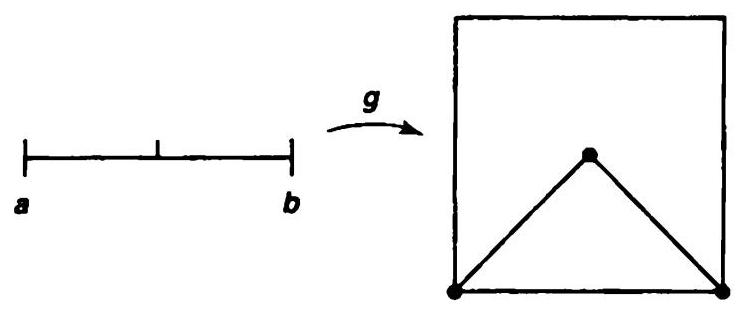
\includegraphics[width=0.6\textwidth]{images/44.1.jpg}
\end{center}
\hspace*{3em} 

Figure 44.1

\begin{center}
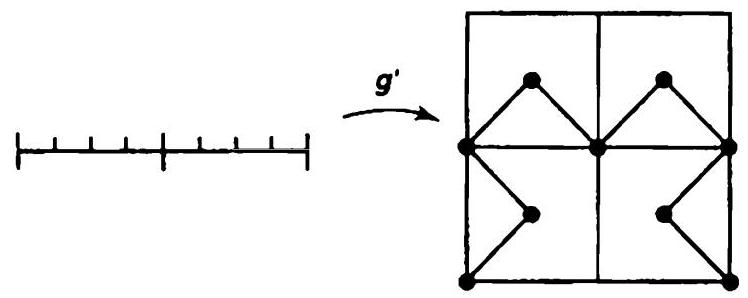
\includegraphics[width=0.6\textwidth]{images/44.2.jpg}
\end{center}
\hspace*{3em} 

Figure 44.2

This same operation can also be applied to any triangular path connecting two adjacent corners of the square. For instance, when applied to the path \(h\) pictured in Figure 443, it gives the path \({h}^{\prime }\)

Step 2. Now we define a sequence of functions \({f}_{n} : I \rightarrow  {I}^{2}\) . The first function, which we label \({f}_{0}\) for convenience, is the triangular path pictured in Figure 44.1, letting \(a = 0\) and \(b = 1\) . The next function \({f}_{1}\) is the function obtained by applying the operation described in Step 1 to the function \({f}_{0}\) ; it is pictured in Figure 44.2. The next function \({f}_{2}\) is the function obtained by applying this same operation to each of the four

\begin{center}
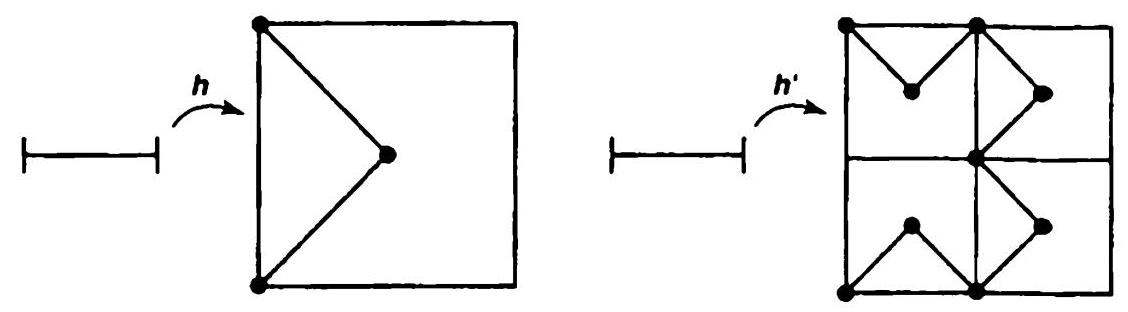
\includegraphics[width=1.0\textwidth]{images/44.3.jpg}
\end{center}
\hspace*{3em} 

Figure 44.3

triangular paths that make up \({f}_{1}\) . It is pictured in Figure 44.4. The next function \({f}_{3}\) is obtained by applying the operation to each of the 16 triangular paths that make up \({f}_{2}\) ; it is pictured in Figure 44.5. And so on. At the general step, \({f}_{n}\) is a path made up of \({4}^{n}\) triangular paths of the type considered in Step 1, each lying in a square of edge length \(1/{2}^{n}\) . The function \({f}_{n + 1}\) is obtained by applying the operation of Step1 to these triangular paths, replacing each one by four smaller triangular paths.

\begin{center}
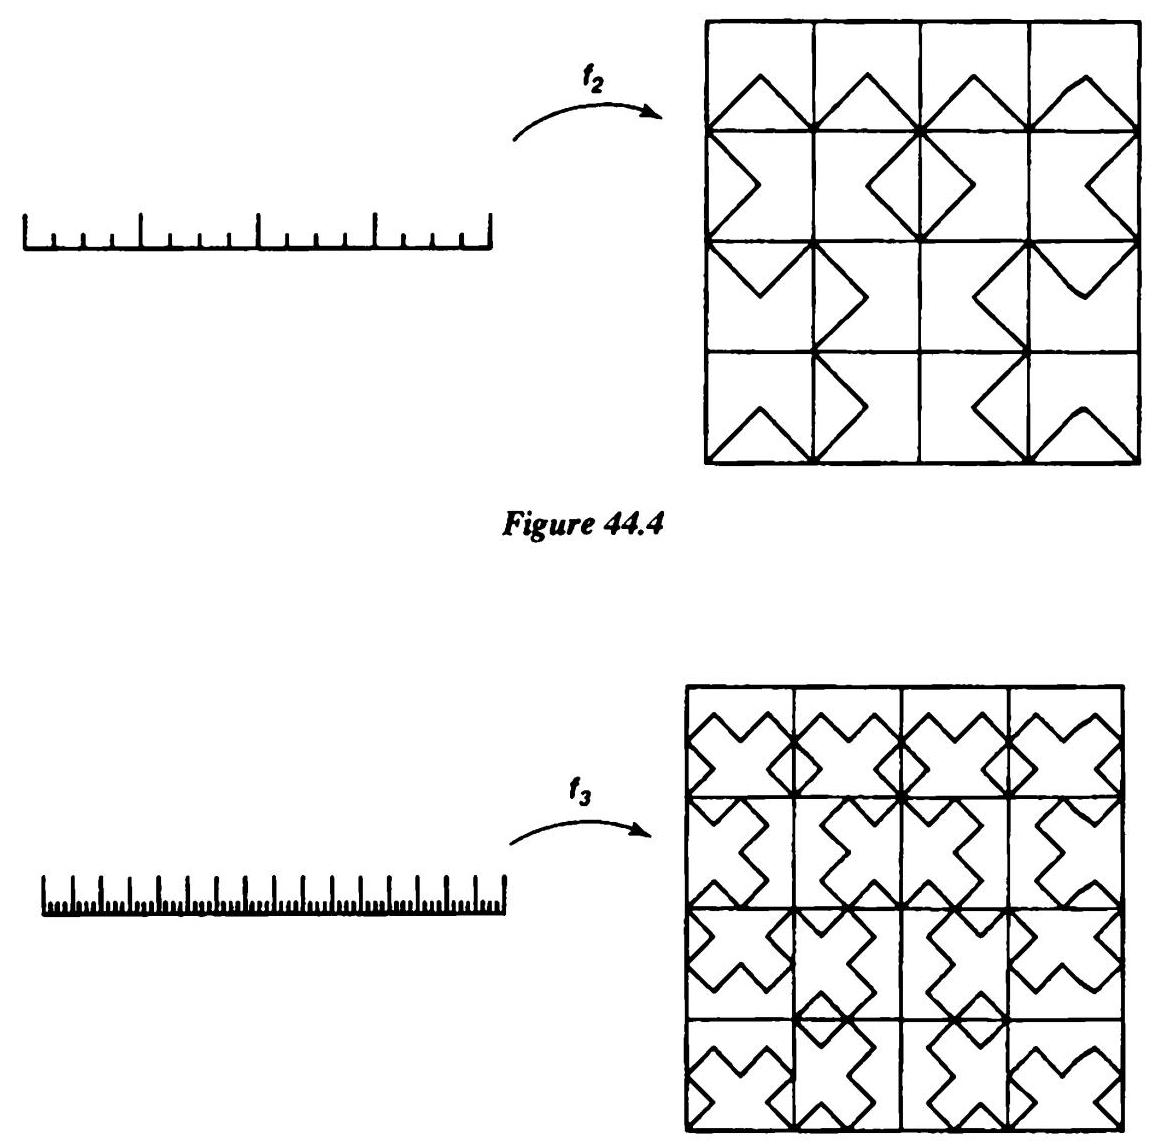
\includegraphics[width=1.0\textwidth]{images/44.4.jpg}
\end{center}
\hspace*{3em} 

Figure 44.5

Step 3. For purposes of this proof, let \(d\left( {\mathbf{x},\mathbf{y}}\right)\) denote the square metric on \({\mathbb{R}}^{2}\) ,

\[
d\left( {\mathbf{x},\mathbf{y}}\right)  = \max \left\{  {\left| {{x}_{1} - {y}_{1}}\right| ,\left| {{x}_{2} - {y}_{2}}\right| }\right\}  .
\]

Then we can let \(\rho\) denote the corresponding sup metric on \(\mathcal{C}\left( {I,{I}^{2}}\right)\) :

\[
\rho \left( {f,g}\right)  = \sup \{ d\left( {f\left( t\right) ,g\left( t\right) }\right)  \mid  t \in  I\} .
\]

Because \({I}^{2}\) is closed in \({\mathbb{R}}^{2}\) , it is complete in the square metric; then \(\mathcal{C}\left( {I,{I}^{2}}\right)\) is complete in the metric \(\rho\) .

We assert that the sequence of functions \(\left( {f}_{n}\right)\) defined in Step 2 is a Cauchy sequence under \(\rho\) . To prove this fact, let us examine what happens when we pass from \({f}_{n}\) to \({f}_{n + 1}\) . Each of the small triangular paths that make up \({f}_{n}\) lies in a square of edge length \(1/{2}^{n}\) . The operation by which we obtain \({f}_{n + 1}\) replaces each such triangular path by four triangular paths that lie in the same square. Therefore, in the square metric on \({I}^{2}\) , the distance between \({f}_{n}\left( t\right)\) and \({f}_{n + 1}\left( t\right)\) is at most \(1/{2}^{n}\) . As a result, \(\rho \left( {{f}_{n},{f}_{n + 1}}\right)  \leq  1/{2}^{n}\) . It follows that \(\left( {f}_{n}\right)\) is a Cauchy sequence, since

\[
\rho \left( {{f}_{n},{f}_{n + m}}\right)  \leq  1/{2}^{n} + 1/{2}^{n + 1} + \cdots  + 1/{2}^{n + m - 1} < 2/{2}^{n}
\]

for all \(n\) and \(m\) .

Step 4. Because \(\mathcal{C}\left( {I,{I}^{2}}\right)\) is complete, the sequence \({f}_{n}\) converges to a continuous function \(f : I \rightarrow  {I}^{2}\) . We prove that \(f\) is surjective.

Let \(x\) be a point of \({I}^{2}\) ; we show that \(x\) belongs to \(f\left( I\right)\) . First we note that, given \(n\) , the path \({f}_{n}\) comes within a distance of \(1/{2}^{n}\) of the point \(\mathbf{x}\) . For the path \({f}_{n}\) touches each of the little squares of edge length \(1/{2}^{n}\) into which we have divided \({I}^{2}\) .

Using this fact, we shall prove that, given \(\epsilon  > 0\) , the \(\epsilon\) -neighborhood of \(\mathbf{x}\) intersects \(f\left( I\right)\) . Choose \(N\) large enough that

\[
\rho \left( {{f}_{N},f}\right)  < \epsilon /2\;\text{ and }\;1/{2}^{N} < \epsilon /2.
\]

By the result of the previous paragraph, there is a point \({t}_{0} \in  I\) such that \(d\left( {\mathbf{x},{f}_{N}\left( {t}_{0}\right) }\right)  \leq\)  \(1/{2}^{N}\) . Then since \(d\left( {{f}_{N}\left( t\right) ,f\left( t\right) }\right)  < \epsilon /2\) for all \(t\) , it follows that

\[
d\left( {\mathbf{x},f\left( {t}_{0}\right) }\right)  < \epsilon ,
\]

so the \(\epsilon\) -neighborhood of \(\mathbf{x}\) intersects \(f\left( I\right)\) .

It follows that \(\mathbf{x}\) belongs to the closure of \(f\left( I\right)\) . But \(I\) is compact, so \(f\left( I\right)\) is compact and is therefore closed. Hence \(\mathbf{x}\) lies in \(f\left( I\right)\) , as desired.
\end{proof}
\section*{Exercises}

1. Given \(n\) , show there is a continuous surjective map \(g : I \rightarrow  {I}^{n}\) . [Hint: Consider \(\left. {f \times  f \cdot  I \times  I \rightarrow  {I}^{2} \times  {I}^{2}.}\right\rbrack\)

2. Show there is a continuous surjective map \(f : \mathbb{R} \rightarrow  {\mathbb{R}}^{n}\) .

3. (a) If \({\mathbb{R}}^{\omega }\) is given the product topology, show there is no continuous surjective map \(f : \mathbb{R} \rightarrow  {\mathbb{R}}^{\omega }\) . [Hint: Show that \({\mathbb{R}}^{\omega }\) is not a countable union of compact subspaces.]

(b) If \({\mathbb{R}}^{\omega }\) is given the product topology, determine whether or not there is a continuous surjective map of \(\mathbb{R}\) onto the subspace \({\mathbb{R}}^{\infty }\) .

(c) What happens to the statements in (a) and (b) if \({\mathbb{R}}^{\omega }\) is given the uniform topology or the box topology?

4. (a) Let \(X\) be a Hausdorff space. Show that if there is a continuous surjective map \(f : I \rightarrow  X\) , then \(X\) is compact, connected, weakly locally connected, and metrizable. [Hint: Show \(f\) is a perfect map.]

(b) The converse of the result in (a) is a famous theorem of point-set topology called the \idx{Hahn-Mazurkiewicz theorem} (see 		\cite{HockingYoung1961}, p. 129). Assuming this theorem, show there is a continuous surjective map \(f \cdot  I \rightarrow  {I}^{\omega }\) .

A Hausdorff space that is the continuous image of the closed unit interval is often called a \idx{Peano space} Peano space.

\section*{§ 45 Compactness in Metric Spaces}

We have already shown that compactness, limit point compactness, and sequential compactness are equivalent for metric spaces. There is still another formulation of compactness for metric spaces, one that involves the notion of completeness. We study it in this section. As an application, we shall prove a theorem characterizing those subspaces of \(\mathcal{C}\left( {X,{\mathbb{R}}^{n}}\right)\) that are compact in the uniform topology.

How is compactness of a metric space \(X\) related to completeness of \(X\) ? It follows from Lemma 431 that every compact metric space is complete. The converse does not hold-a complete metric space need not be compact. It is reasonable to ask what extra condition one needs to impose on a complete space to be assured of its compactness. Such a condition is the one called total boundedness.

\begin{definition} A metric space(X, d)is said to be \idx{totally bounded} if for every \(\epsilon  > 0\) , there is a finite covering of \(X\) by \(\epsilon\) -balls.
\end{definition}

\begin{example} Total boundedness clearly implies boundedness. For if \(B\left( {{x}_{1},1/2}\right) ,\ldots\) , \(B\left( {{x}_{n},1/2}\right)\) is a finite covering of \(X\) by open balls of radius \(1/2\) , then \(X\) has diameter at most \(1 + \max \left\{  {d\left( {{x}_{i},{x}_{j}}\right) }\right\}\) . The converse does not hold, however. For example, in the metric \(\bar{d}\left( {a,b}\right)  = \min \{ 1,\left| {a - b}\right| \}\) , the real line \(\mathbb{R}\) is bounded but not totally bounded.
\end{example}

\begin{example} Under the metric \(d\left( {a,b}\right)  = \left| {a - b}\right|\) , the real line \(\mathbb{R}\) is complete but not totally bounded, while the subspace(-1,1)is totally bounded but not complete. The subspace \(\left\lbrack  {-1,1}\right\rbrack\) is both complete and totally bounded.
\end{example}

\begin{theorem} A metric space(X, d)is compact if and only if it is complete and totally bounded.
\end{theorem}

\begin{proof}If \(X\) is a compact metric space, then \(X\) is complete, as noted above. The fact that \(X\) is totally bounded is a consequence of the fact that the covering of \(X\) by all open \(\epsilon\) -balls must contain a finite subcovering.
Conversely, let \(X\) be complete and totally bounded. We shall prove that \(X\) is sequentially compact. This will suffice.

Let \(\left( {x}_{n}\right)\) be a sequence of points of \(X\) . We shall construct a subsequence of \(\left( {x}_{n}\right)\) that is a Cauchy sequence, so that it necessarily converges. First cover \(X\) by finitely many balls of radius 1 . At least one of these balls, say \({B}_{1}\) , contains \({x}_{n}\) for infinitely many values of \(n\) . Let \({J}_{1}\) be the subset of \({\mathbb{Z}}_{ + }\) consisting of those indices \(n\) for which \({x}_{n} \in  {B}_{1}\) .

Next, cover \(X\) by finitely many balls of radius \(1/2\) . Because \({J}_{1}\) is infinite, at least one of these balls, say \({B}_{2}\) , must contain \({x}_{n}\) for infinitely many values of \(n\) in \({J}_{1}\) . Choose \({J}_{2}\) to be the set of those indices \(n\) for which \(n \in  {J}_{1}\) and \({x}_{n} \in  {B}_{2}\) . In general, given an infinite set \({J}_{k}\) of positive integers, choose \({J}_{k + 1}\) to be an infinite subset of \({J}_{k}\) such that there is a ball \({B}_{k + 1}\) of radius \(1/\left( {k + 1}\right)\) that contains \({x}_{n}\) for all \(n \in  {J}_{k + 1}\) .

Choose \({n}_{1} \in  {J}_{1}\) . Given \({n}_{k}\) , choose \({n}_{k + 1} \in  {J}_{k + 1}\) such that \({n}_{k + 1} > {n}_{k}\) ; this we can do because \({J}_{k + 1}\) is an infinite set. Now for \(i,j \geq  k\) , the indices \({n}_{i}\) and \({n}_{j}\) both belong to \({J}_{k}\) (because \({J}_{1} \supset  {J}_{2} \supset  \cdots\) is a nested sequence of sets). Therefore, for all \(i,j \geq  k\) , the points \({x}_{{n}_{i}}\) and \({x}_{{n}_{j}}\) are contained in a ball \({B}_{k}\) of radius \(1/k\) . It follows that the sequence \(\left( {x}_{{n}_{1}}\right)\) is a Cauchy sequence, as desired.

We now apply this result to find the compact subspaces of the space \(\mathcal{C}\left( {X,{\mathbb{R}}^{n}}\right)\) , in the uniform topology. We know that a subspace of \({\mathbb{R}}^{n}\) is compact if and only if it is closed and bounded. One might hope that an analogous result holds for \(\mathcal{C}\left( {X,{\mathbb{R}}^{n}}\right)\) . But it does not, even if \(X\) is compact. One needs to assume that the subspace of \(\mathcal{C}\left( {X,{\mathbb{R}}^{n}}\right)\) satisfies an additional condition, called \idx{equicontinuity}. We consider that notion now.
\end{proof}
\begin{definition} Let(Y, d)be a metric space. Let \(\mathcal{F}\) be a subset of the function space \(\mathcal{C}\left( {X,Y}\right)\) . If \({x}_{0} \in  X\) , the set \(\mathcal{F}\) of functions is said to be equicontinuous at \({x}_{0}\) if given \(\epsilon  > 0\) , there is a neighborhood \(U\) of \({x}_{0}\) such that for all \(x \in  U\) and all \(f \in  \mathcal{F}\) ,

\[
d\left( {f\left( x\right) ,f\left( {x}_{0}\right) }\right)  < \epsilon
\]

If the set \(\mathcal{F}\) is equicontinuous at \({x}_{0}\) for each \({x}_{0} \in  X\) , it is said simply to be equicontinuous.
\end{definition}

Continuity of the function \(f\) at \({x}_{0}\) means that given \(f\) and given \(\epsilon  > 0\) , there exists a neighborhood \(U\) of \({x}_{0}\) such that \(d\left( {f\left( x\right) ,f\left( {x}_{0}\right) }\right)  < \epsilon\) for \(x \in  U\) . Equicontinuity of \(\mathcal{F}\) means that a single neighborhood \(U\) can be chosen that will work for all the functions \(f\) in the collection \(\mathcal{F}\) .

Note that equicontinuity depends on the specific metric \(d\) rather than merely on the topology of \(Y\) .

\begin{lemma} Let \(X\) be a space; let(Y, d)be a metric space. If the subset \(\mathcal{F}\) of \(\mathcal{C}\left( {X,Y}\right)\) is totally bounded under the uniform metric corresponding to \(d\) , then \(\mathcal{F}\) is equicontinuous under \(d\) .
\end{lemma}

\begin{proof}Assume \(\mathcal{F}\) is totally bounded. Given \(0 < \epsilon  < 1\) , and given \({x}_{0}\) , we find a neighborhood \(U\) of \({x}_{0}\) such that \(d\left( {f\left( x\right) ,f\left( {x}_{0}\right)  < \epsilon }\right.\) for \(x \in  U\) and \(f \in  \mathcal{F}\) .
Set \(\delta  = \epsilon /3\) ; cover \(\mathcal{F}\) by finitely many open \(\delta\) -balls

\[
B\left( {{f}_{1},\delta }\right) ,\ldots ,B\left( {{f}_{n},\delta }\right)
\]

in \(\mathcal{C}\left( {X,Y}\right)\) . Each function \({f}_{i}\) is continuous; therefore, we can choose a neighborhood \(U\) of \({x}_{0}\) such that for \(i = 1,\ldots ,n\) ,

\[
d\left( {{f}_{i}\left( x\right) ,{f}_{i}\left( {x}_{0}\right) }\right)  < \delta
\]

whenever \(x \in  U\) .

Let \(f\) be an arbitrary element of \(\mathcal{F}\) . Then \(f\) belongs to at least one of the above \(\delta\) -balls, say to \(B\left( {{f}_{i},\delta }\right)\) . Then for \(x \in  U\) , we have

\[
\bar{d}\left( {f\left( x\right) ,{f}_{i}\left( x\right) }\right)  < \delta ,
\]

\[
d\left( {{f}_{i}\left( x\right) ,{f}_{i}\left( {x}_{0}\right) }\right)  < \delta ,
\]

\[
\bar{d}\left( {{f}_{i}\left( {x}_{0}\right) ,f\left( {x}_{0}\right) }\right)  < \delta .
\]

The first and third inequalities hold because \(\bar{\rho }\left( {f,{f}_{i}}\right)  < \delta\) , and the second holds because \(x \in  U\) . Since \(\delta  < 1\) , the first and third also hold if \(\bar{d}\) is replaced by \(d\) ; then the triangle inequality implies that for all \(x \in  U\) , we have \(d\left( {f\left( x\right) ,f\left( {x}_{0}\right) }\right)  < \epsilon\) , as desired.

Now we prove the classical version of \idx{Ascoli's theorem}, which concerns compact subspaces of the function space \(\mathcal{C}\left( {X,{\mathbb{R}}^{n}}\right)\) . A more general version, whose proof does not depend on this one, is given in §47. The general version, however, relies on the Tychonoff theorem, whereas this one does not.

We begin by proving a partial converse to the preceding lemma, which holds when \(X\) and \(Y\) are compact.

*Lemma 45.3. Let \(X\) be a space; let(Y, d)be a metric space; assume \(X\) and \(Y\) are compact. If the subset \(\mathcal{F}\) of \(\mathcal{C}\left( {X,Y}\right)\) is equicontinuous under \(d\) , then \(\mathcal{F}\) is totally bounded under the uniform and sup metrics corresponding to \(d\) .

Proof. Since \(X\) is compact, the sup metric \(\rho\) is defined on \(\mathcal{C}\left( {X,Y}\right)\) . Total boundedness under \(\rho\) is equivalent to total boundedness under \(\bar{\rho }\) , for whenever \(\epsilon  < 1\) , every \(\epsilon\) -ball under \(\rho\) is also an \(\epsilon\) -ball under \(\bar{\rho }\) , and conversely. Therefore, we may as well use the metric \(\rho\) throughout.

Assume \(\mathcal{F}\) is equicontinuous. Given \(\epsilon  > 0\) , we cover \(\mathcal{F}\) by finitely many sets that are open \(\epsilon\) -balls in the metric \(\rho\) .

Set \(\delta  = \epsilon /3\) . Given any \(a \in  X\) , there is a corresponding neighborhood \({U}_{a}\) of \(a\) such that \(d\left( {f\left( x\right) ,f\left( a\right) }\right)  < \delta\) for all \(x \in  {U}_{a}\) and all \(f \in  \mathcal{F}\) . Cover \(X\) by finitely many such neighborhoods \({U}_{a}\) , for \(a = {a}_{1},\ldots ,{a}_{k}\) , denote \({U}_{{a}_{i}}\) by \({U}_{i}\) . Then cover \(Y\) by finitely many open sets \({V}_{1},\ldots ,{V}_{m}\) of diameter less than \(\delta\) .

Let \(J\) be the collection of all functions \(\alpha  : \{ 1,\ldots ,k\}  \rightarrow  \{ 1,\ldots ,m\}\) . Given \(\alpha  \in  J\) , if there exists a function \(f\) of \(\mathcal{F}\) such that \(f\left( {a}_{i}\right)  \in  {V}_{\alpha \left( i\right) }\) for each \(i = 1,\ldots ,k\) , choose one such function and label it \({f}_{\alpha }\) . The collection \(\left\{  {f}_{\alpha }\right\}\) is indexed by a subset \({J}^{\prime }\) of the set \(J\) and is thus finite We assert that the open balls \({B}_{\rho }\left( {{f}_{\alpha },\epsilon }\right)\) , for \(\alpha  \in  {J}^{\prime }\) , cover \(\mathcal{F}\) .

Let \(f\) be an element of \(\mathcal{F}\) . For each \(i = 1,\ldots ,k\) , choose an integer \(\alpha \left( i\right)\) such that \(f\left( {a}_{i}\right)  \in  {V}_{\alpha \left( i\right) }\) . Then the function \(\alpha\) is in \({J}^{\prime }\) . We assert that \(f\) belongs to the ball \({B}_{\rho }\left( {{f}_{\alpha },\epsilon }\right)\) .

Let \(x\) be a point of \(X\) . Choose \(i\) so that \(x \in  {U}_{i}\) . Then

\[
d\left( {f\left( x\right) ,f\left( {a}_{l}\right) }\right)  < \delta ,
\]

\[
d\left( {f\left( {a}_{i}\right) ,{f}_{\alpha }\left( {a}_{i}\right) }\right)  < \delta ,
\]

\[
d\left( {{f}_{\alpha }\left( {a}_{i}\right) ,{f}_{\alpha }\left( x\right) }\right)  < \delta .
\]

The first and third inequalities hold because \(x \in  {U}_{i}\) , and the second holds because \(f\left( {a}_{i}\right)\) and \({f}_{\alpha }\left( {a}_{i}\right)\) are in \({V}_{\alpha \left( i\right) }\) . We conclude that \(d\left( {f\left( x\right) ,{f}_{\alpha }\left( x\right) }\right)  < \epsilon\) . Because this inequality holds for every \(x \in  X\) ,

\[
\rho \left( {f,{f}_{\alpha }}\right)  = \max \left\{  {d\left( {f\left( x\right) ,{f}_{\alpha }\left( x\right) }\right) }\right\}   < \epsilon .
\]

Thus \(f\) belongs to \({B}_{\rho }\left( {{f}_{\alpha },\epsilon }\right)\) , as asserted.
\end{proof}
\begin{definition} If(Y, d)is a metric space, a subset \(\mathcal{F}\) of \(\mathcal{C}\left( {X,Y}\right)\) is said to be \idx{pointwise bounded} under \(d\) if for each \(x \in  X\) , the subset

\[
{\mathcal{F}}_{a} = \{ f\left( a\right)  \mid  f \in  \mathcal{F}\}
\]

of \(Y\) is bounded under \(d\) .
\end{definition}

*Theorem 45.4 (Ascoli’s theorem, classical version). Let \(X\) be a compact space; let \(\left( {{\mathbb{R}}^{n},d}\right)\) denote euclidean space in either the square metric or the euclidean metric; give \(\mathcal{C}\left( {X,{\mathbb{R}}^{n}}\right)\) the corresponding uniform topology. A subspace \(\mathcal{F}\) of \(\mathcal{C}\left( {X,{\mathbb{R}}^{n}}\right)\) has compact closure if and only if \(\mathcal{F}\) is equicontinuous and pointwise bounded under \(d\) .

\begin{proof}Since \(X\) is compact, the sup metric \(\rho\) is defined on \(\mathcal{C}\left( {X,{\mathbb{R}}^{n}}\right)\) and gives the uniform topology on \(\mathcal{C}\left( {X,{\mathbb{R}}^{n}}\right)\) . Throughout, let \(\mathcal{G}\) denote the closure of \(\mathcal{F}\) in \(C\left( {X,{\mathbb{R}}^{n}}\right)\) .
Step 1. We show that if \(g\) is compact, then \(g\) is equicontinuous and pointwise bounded under \(d\) . Since \(\mathcal{F} \subset  \mathcal{G}\) , it follows that \(\mathcal{F}\) is also equicontinuous and pointwise bounded under \(d\) . This proves the "only if" part of the theorem.

Compactness of \(\mathcal{G}\) implies that \(\mathcal{G}\) is totally bounded under \(\rho\) and \(\bar{\rho }\) by Theorem 45.1, this in turn implies that \(\mathcal{G}\) is equicontinuous under \(d\) , by Lemma 45.2. Compactness of \(\mathcal{G}\) also implies that \(\mathcal{G}\) is bounded under \(\rho\) ; this in turn implies that \(\mathcal{G}\) is pointwise bounded under \(d\) . For if \(\rho \left( {f,g}\right)  \leq  M\) for all \(f,g \in  \mathcal{G}\) , then in particular \(d\left( {f\left( a\right) ,g\left( a\right) }\right)  \leq  M\) for \(f,g \in  \mathcal{G}\) , so that \({\mathcal{G}}_{a}\) has diameter at most \(M\) .

Step 2. We show that if \(\mathcal{F}\) is equicontinuous and pointwise bounded under \(d\) , then so is \(g\) .

First, we check equicontinuity. Given \({x}_{0} \in  X\) and given \(\epsilon  > 0\) , choose a neighborhood \(U\) of \({x}_{0}\) such that \(d\left( {f\left( x\right) ,f\left( {x}_{0}\right) }\right)  < \epsilon /3\) for all \(x \in  U\) and \(f \in  \mathcal{F}\) . Given \(g \in  \mathcal{G}\) , choose \(f \in  \mathcal{F}\) so that \(\rho \left( {f,g}\right)  < \epsilon /3\) The triangle inequality implies that \(d\left( {g\left( x\right) ,g\left( {x}_{0}\right) }\right)  < \epsilon\) for all \(x \in  U\) . Since \(g\) is arbitrary, equicontinuity of \(\mathcal{G}\) at \({x}_{0}\) follows.

Second, we verify pointwise boundedness. Given \(a\) , choose \(M\) so that \(\operatorname{diam}{\mathcal{F}}_{a} \leq\)  \(M\) . Then, given \(g,{g}^{\prime } \in  \mathcal{G}\) , choose \(f,{f}^{\prime } \in  \mathcal{F}\) such that \(\rho \left( {f,g}\right)  < 1\) and \(\rho \left( {{f}^{\prime },{g}^{\prime }}\right)  < 1\) . Since \(d\left( {f\left( a\right) ,{f}^{\prime }\left( a\right) }\right)  \leq  M\) , it follows that \(d\left( {g\left( a\right) ,{g}^{\prime }\left( a\right) }\right)  \leq  M + 2\) . Then since \(g\) and \({g}^{\prime }\) are arbitrary, it follows that diam \({\mathcal{G}}_{a} \leq  M + 2\) .

Step 3. We show that if \(\xi\) is equicontinuous and pointwise bounded, then there is a compact subspace \(Y\) of \({\mathbb{R}}^{n}\) that contains the union of the sets \(g\left( X\right)\) , for \(g \in  \mathcal{G}\) .

Choose, for each \(a \in  X\) , a neighborhood \({U}_{a}\) of \(a\) such that \(d\left( {g\left( x\right) ,g\left( a\right) }\right)  < 1\) for \(x \in  {U}_{a}\) and \(g \in  \mathcal{G}\) . Since \(X\) is compact, we can cover \(X\) by finitely many such neighborhoods, say for \(a = {a}_{1},\ldots ,{a}_{k}\) . Because the sets \({\mathcal{G}}_{{a}_{i}}\) are bounded, their union is also bounded; suppose it lies in the ball of radius \(N\) in \({\mathbb{R}}^{n}\) centered at the origin. Then for all \(g \in  \mathcal{G}\) , the set \(g\left( X\right)\) is contained in the ball of radius \(N + 1\) centered at the origin. Let \(Y\) be the closure of this ball.

Step 4. We prove the "if" part of the theorem. Assume that \(\mathcal{F}\) is equicontinuous and pointwise bounded under \(d\) . We show that \(\mathcal{G}\) is complete and totally bounded under \(\rho\) ; then Theorem 45.1 implies that \(\mathcal{G}\) is compact.

Completeness is easy, for \(\mathcal{G}\) is a closed subspace of the complete metric space \(\left( {C\left( {X,{\mathbb{R}}^{n}}\right) ,\rho }\right)\) .

We verify total boundedness. First, Step 2 implies that \(\mathcal{G}\) is equicontinuous and pointwise bounded under \(d\) ; then Step 3 tells us that there is a compact subspace \(Y\) of \({\mathbb{R}}^{n}\) such that \(\mathcal{G} \subset  \mathcal{C}\left( {X,Y}\right)\) . Equicontinuity of \(\mathcal{G}\) now implies, by Lemma 45.3, that \(\mathcal{G}\) is totally bounded under \(\rho\) , as desired.

*Corollary 45.5. Let \(X\) be compact; let \(d\) denote either the square metric or the euclidean metric on \({\mathbb{R}}^{n}\) ; give \(\mathcal{C}\left( {X,{\mathbb{R}}^{n}}\right)\) the corresponding uniform topology. A subspace \(\mathcal{F}\) of \(\mathcal{C}\left( {X,{\mathbb{R}}^{n}}\right)\) is compact if and only if it is closed, bounded under the sup metric \(\rho\) , and equicontinuous under \(d\) .

Proof. If \(\mathcal{F}\) is compact, it must be closed and bounded; the preceding theorem implies that it is also equicontinuous. Conversely, if \(\mathcal{F}\) is closed, it equals its closure \(\mathcal{G}\) ; if it is bounded under \(\rho\) , it is pointwise bounded under \(d\) ; and if it is also equicontinuous, the preceding theorem implies that it is compact.
\end{proof}
\section*{Exercises}

1. If \({X}_{n}\) is metrizable with metric \({d}_{n}\) , then

\[
D\left( {\mathbf{x},\mathbf{y}}\right)  = \sup \left\{  {{\bar{d}}_{i}\left( {{x}_{i},{y}_{i}}\right) /i}\right\}
\]

is a metric for the product space \(X = \prod {X}_{n}\) . Show that \(X\) is totally bounded under \(D\) if each \({X}_{n}\) is totally bounded under \({d}_{n}\) . Conclude without using the Ty-chonoff theorem that a countable product of compact metrizable spaces is compact.

2. Let(Y, d)be a metric space; let \(\mathcal{F}\) be a subset of \(\mathcal{C}\left( {X,Y}\right)\) .

(a) Show that if \(\mathcal{F}\) is finite, then \(\mathcal{F}\) is equicontinuous.

(b) Show that if \({f}_{n}\) is a sequence of elements of \(\mathcal{C}\left( {X,Y}\right)\) that converges uniformly, then the collection \(\left\{  {f}_{n}\right\}\) is equicontinuous.

(c) Suppose that \(\mathcal{F}\) is a collection of differentiable functions \(f : \mathbb{R} \rightarrow  \mathbb{R}\) such that each \(x \in  \mathbb{R}\) lies in a neighborhood \(U\) on which the derivatives of the functions in \(\mathcal{F}\) are uniformly bounded. \{This means that there is an \(M\) such that \(\left| {{f}^{\prime }\left( x\right) }\right|  \leq  M\) for all \(f\) in \(\mathcal{F}\) and all \(x \in  U\) .] Show that \(\mathcal{F}\) is equicontinuous.

3. Prove the following:

\begin{theorem}[\idx{Arzela’s theorem} Arzela’s theorem] Let \(X\) be compact; let \({f}_{n} \in  \mathcal{C}\left( {X,{\mathbb{R}}^{k}}\right)\) . If the collection \(\left\{  {f}_{n}\right\}\) is pointwise bounded and equicontinuous, then the sequence \({f}_{n}\) has a uniformly convergent subsequence.
\end{theorem}

4. (a) Let \({f}_{n} : I \rightarrow  \mathbb{R}\) be the function \({f}_{n}\left( x\right)  = {x}^{n}\) . The collection \(\mathcal{F} = \left\{  {f}_{n}\right\}\) is pointwise bounded but the sequence \(\left( {f}_{n}\right)\) has no uniformly convergent subsequence; at what point or points does \(\mathcal{F}\) fail to be equicontinuous?

(b) Repeat (a) for the functions \({f}_{n}\) of Exercise 9 of \(§{21}\) .

5. Let \(X\) be a space. A subset \(\mathcal{F}\) of \(\mathcal{C}\left( {X,\mathbb{R}}\right)\) is said to vanish uniformly at infinity if given \(\epsilon  > 0\) , there is a compact subspace \(C\) of \(X\) such that \(\left| {f\left( x\right) }\right|  < \epsilon\) for \(x \in  X - C\) and \(f \in  \mathcal{F}\) If \(\mathcal{F}\) consists of a single function \(f\) , we say simply that \(f\) vanishes at infinity. Let \({\mathcal{C}}_{0}\left( {X,\mathbb{R}}\right)\) denote the set of continuous functions \(f : X \rightarrow  \mathbb{R}\) that \idx{vanish at infinity}.

\begin{theorem} Let \(X\) be locally compact Hausdorff; give \({\mathcal{C}}_{0}\left( {X,\mathbb{R}}\right)\) the uniform topology. A subset \(\mathcal{F}\) of \({\mathcal{C}}_{0}\left( {X,\mathbb{R}}\right)\) has compact closure if and only if it is pointwise bounded, equicontinuous, and vanishes uniformly at infinity.
\end{theorem}

\{Hint: Let \(Y\) denote the one-point compactification of \(X\) . Show that \({\mathcal{C}}_{0}\left( {X,\mathbb{R}}\right)\) is isometric with a closed subspace of \(\mathcal{C}\left( {Y,\mathbb{R}}\right)\) if both are given the sup metric.]

6. Show that our proof of Ascoli’s theorem goes through if \({\mathbb{R}}^{n}\) is replaced by any metric space in which all closed bounded subspaces are compact.

*7. Let(X, d)be a metric space. If \(A \subset  X\) and \(\epsilon  > 0\) , let \(U\left( {A,\epsilon }\right)\) be the \(\epsilon\) - neighborhood of \(A\) . Let \(\mathcal{H}\) be the collection of all (nonempty) closed, bounded subsets of \(X\) . If \(A,B \in  \mathcal{H}\) , define

\[
D\left( {A,B}\right)  = \inf \{ \epsilon  \mid  A \subset  U\left( {B,\epsilon }\right) \text{ and }B \subset  U\left( {A,\epsilon }\right) \} .
\]

(a) Show that \(D\) is a metric on \(\mathcal{H}\) ; it is called the \idx{Hausdorff metric}.

(b) Show that if(X, d)is complete, so is(H, D). [Hint: Let \({A}_{n}\) be a Cauchy sequence in \(\mathcal{H}\) ; by passing to a subsequence, assume \(D\left( {{A}_{n},{A}_{n + 1}}\right)  < 1/{2}^{n}\) . Define \(A\) to be the set of all points \(x\) that are the limits of sequences \({x}_{1},{x}_{2}\) , ... such that \({x}_{i} \in  {A}_{i}\) for each \(i\) and \(d\left( {{x}_{i},{x}_{i + 1}}\right)  < 1/{2}^{i}\) . Show \(\left. {{A}_{n} \rightarrow  \bar{A}\text{ . }}\right\rbrack\)

(c) Show that if(X, d)is totally bounded, so is(H, D). [Hint: Given \(\epsilon\) , choose \(\delta  < \epsilon\) and let \(S\) be a finite subset of \(X\) such that the collection \(\left\{  {{B}_{d}\left( {x,\delta }\right)  \mid  }\right.\)  \(x \in  S\}\) covers \(X\) . Let \(\mathcal{A}\) be the collection of all nonempty subsets of \(S\) ; show that \(\left\{  {{B}_{D}\left( {A,\epsilon }\right)  \mid  A \in  \mathcal{A}}\right\}\) covers \(\mathcal{H}\) .]

(d) Theorem. If \(X\) is compact in the metric \(d\) , then the space \(\mathcal{H}\) is compact in the Hausdorff metric \(D\) .

*8. Let \(\left( {X,{d}_{X}}\right)\) and \(\left( {Y,{d}_{Y}}\right)\) be metric spaces; give \(X \times  Y\) the corresponding square metric; let \(\mathcal{H}\) denote the collection of all nonempty closed, bounded subsets of \(X \times  Y\) in the resulting Hausdorff metric. Consider the space \(\mathcal{C}\left( {X,Y}\right)\) in the uniform metric; let \(\operatorname{gr} : \mathcal{C}\left( {X,Y}\right)  \rightarrow  \mathcal{H}\) be the function that assigns, to each continuous function \(f : X \rightarrow  Y\) , its graph

\[
{G}_{f} = \{ x \times  f\left( x\right)  \mid  x \in  X\} .
\]

(a) Show that the map gr is injective and uniformly continuous.

(b) Let \({\mathcal{H}}_{0}\) denote the image set of the map gr; let \(g : \mathcal{C}\left( {X,Y}\right)  \rightarrow  {\mathcal{H}}_{0}\) be the surjective map obtained from gr. Show that if \(f : X \rightarrow  Y\) is uniformly continuous, then the map \({g}^{-1}\) is continuous at the point \({G}_{f}\) .

(c) Give an example where \({g}^{-1}\) is not continuous at the point \({G}_{f}\) .

(d) Theorem. If \(X\) is compact, then \(\operatorname{gr} : \mathcal{C}\left( {X,Y}\right)  \rightarrow  \mathcal{H}\) is an imbedding.

\section*{§ 46 Pointwise and Compact Convergence}

There are other useful topologies on the spaces \({Y}^{X}\) and \(\mathcal{C}\left( {X,Y}\right)\) in addition to the uniform topology. We shall consider three of them here; they are called the topology of pointwise convergence, the topology of compact convergence, and the \idx{compact-open topology}.

\begin{definition} Given a point \(x\) of the set \(X\) and an open set \(U\) of the space \(Y\) , let

\[
S\left( {x,U}\right)  = \left\{  {f \mid  f \in  {Y}^{\chi }\text{ and }f\left( x\right)  \in  U}\right\}  .
\]

The sets \(S\left( {x,U}\right)\) are a subbasis for topology on \({Y}^{X}\) , which is called the topology of pointwise convergence (or the \idx{point-open topology}).
\end{definition}

The general basis element for this topology is a finite intersection of subbasis elements \(S\left( {x,U}\right)\) . Thus a typical basis element about the function \(f\) consists of all functions \(g\) that are "close" to \(f\) at finitely many points. Such a neighborhood is illustrated in Figure 46.1; it consists of all functions \(g\) whose graphs intersect the three vertical intervals pictured.

\begin{center}
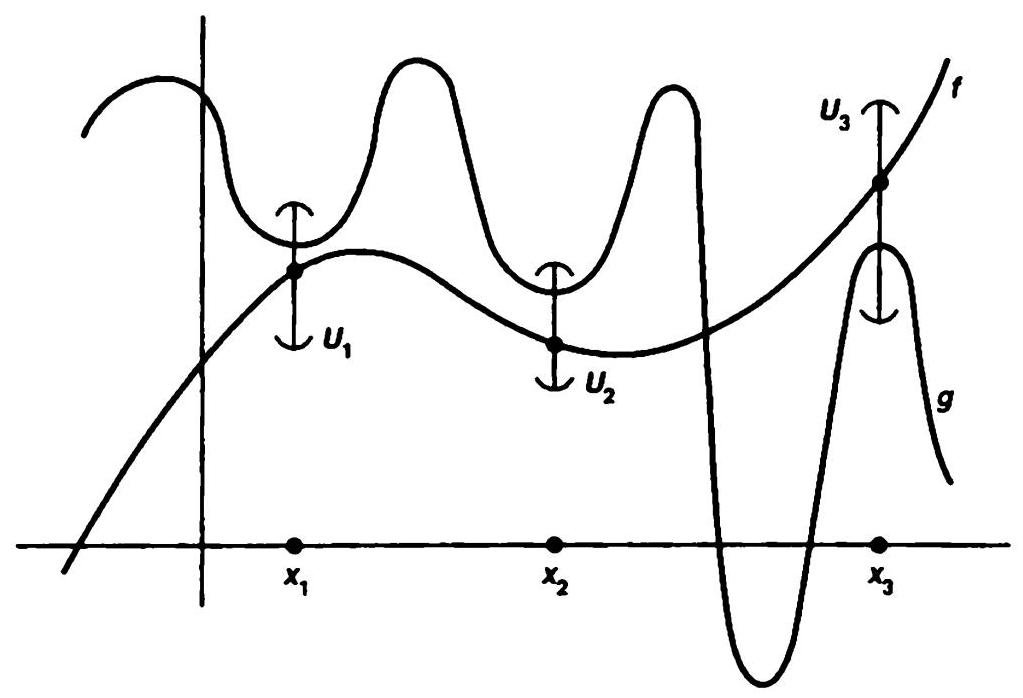
\includegraphics[width=0.9\textwidth]{images/46.1.jpg}
\end{center}
\hspace*{3em} 

Figure 46.1

The topology of pointwise convergence on \({Y}^{X}\) is nothing new. It is just the product topology we have already studied. If we replace \(X\) by \(J\) and denote the general element of \(J\) by \(\alpha\) to make it look more familiar, then the set \(S\left( {\alpha ,U}\right)\) of all functions \(\mathbf{x} : J \rightarrow  Y\) such that \(\mathbf{x}\left( \alpha \right)  \in  U\) is just the subset \({\pi }_{\alpha }^{-1}\left( U\right)\) of \({Y}^{J}\) , which is the standard subbasis element for the product topology.

The reason for calling it the topology of pointwise convergence comes from the following theorem:

\begin{theorem} A sequence \({f}_{n}\) of functions converges to the function \(f\) in the topology of pointwise convergence if and only if for each \(x\) in \(X\) , the sequence \({f}_{n}\left( x\right)\) of points of \(Y\) converges to the point \(f\left( x\right)\) .
\end{theorem}

\begin{proof}This result is just a reformulation, in function space notation, of a standard result about the product topology proved as Lemma 43.3.
\begin{example} Consider the space \({\mathbb{R}}^{I}\) , where \(I = \left\lbrack  {0,1}\right\rbrack\) . The sequence \(\left( {f}_{n}\right)\) of continuous functions given by \({f}_{n}\left( x\right)  = {x}^{n}\) converges in the topology of pointwise convergence to the function \(f\) defined by

\[
f\left( x\right)  = \left\{  \begin{array}{ll} 0 & \text{ for }0 \leq  x < 1 \\  1 & \text{ for }x = 1 \end{array}\right.
\]
\end{example}

This example shows that the subspace \(\mathcal{C}\left( {I,\mathbb{R}}\right)\) of continuous functions is not closed in \({\mathbb{R}}^{I}\) in the topology of pointwise convergence.

We know that a sequence \(\left( {f}_{n}\right)\) of continuous functions that converges in the uniform topology has a continuous limit, and the preceding example shows that a sequence that converges only in the topology of pointwise convergence need not. One can ask whether there is a topology intermediate between these two that will suffice to ensure that the limit of a convergent sequence of continuous functions is continuous. The answer is "yes", assuming the (fairly mild) restriction that the space \(X\) be compactly generated, it will suffice if \({f}_{n}\) converges to \(f\) in the topology of compact convergence, which we now define.
\end{proof}
\begin{definition} Let(Y, d)be a metric space; let \(X\) be a topological space. Given an element \(f\) of \({Y}^{X}\) , a compact subspace \(C\) of \(X\) , and a number \(\epsilon  > 0\) , let \({B}_{C}\left( {f,\epsilon }\right)\) denote the set of all those elements \(g\) of \({Y}^{X}\) for which

\[
\sup \{ d\left( {f\left( x\right) ,g\left( x\right) }\right)  \mid  x \in  C\}  < \epsilon .
\]

The sets \({B}_{C}\left( {f,\epsilon }\right)\) form a basis for a topology on \({Y}^{X}\) . It is called the topology of compact convergence (or sometimes the "topology of uniform convergence on compact sets").
\end{definition}

It is easy to show that the sets \({B}_{C}\left( {f,\epsilon }\right)\) satisfy the conditions for a basis. The crucial step is to note that if \(g \in  {B}_{C}\left( {f,\epsilon }\right)\) , then for

\[
\delta  = \epsilon  - \sup \{ d\left( {f\left( x\right) ,g\left( x\right) }\right)  \mid  x \in  C\} .
\]

we have \({B}_{C}\left( {g,\delta }\right)  \subset  {B}_{C}\left( {f,\epsilon }\right)\) .

The topology of compact convergence differs from the topology of pointwise convergence in that the general basis element containing \(f\) consists of functions that are "close" to \(f\) not just at finitely many points, but at all points of some compact set.

The justification for the choice of terminology comes from the following theorem, whose proof is immediate.

\begin{theorem} A sequence \({f}_{n}\;X \rightarrow  Y\) of functions converges to the function \(f\) in the topology of compact convergence if and only if for each compact subspace \(C\) of \(X\) , the sequence \({f}_{n} \mid  C\) converges uniformly to \(f \mid  C\) .
\end{theorem}

\begin{definition} A space \(X\) is said to be compactly generated if it satisfies the following condition: A set \(A\) is open in \(X\) if \(A \cap  C\) is open in \(C\) for each compact subspace \(C\) of \(X\) .
\end{definition}

This condition is equivalent to requiring that a set \(B\) be closed in \(X\) if \(B \cap  C\) is closed in \(C\) for each compact \(C\) . It is a fairly mild restriction on the space; many familiar spaces are compactly generated. For instance:

Lemma 46.3. If \(X\) is locally compact, or if \(X\) satisfies the first countability axiom, then \(X\) is compactly generated. Proof. Suppose that \(X\) is locally compact. Let \(A \cap  C\) be open in \(C\) for every compact subspace \(C\) of \(X\) . We show \(A\) is open in \(X\) . Given \(x \in  A\) , choose a neighborhood \(U\) of \(x\) that lies in a compact subspace \(C\) of \(X\) . Since \(A \cap  C\) is open in \(C\) by hypothesis, \(A \cap  U\) is open in \(U\) , and hence open in \(X\) . Then \(A \cap  U\) is a neighborhood of \(x\) contained in \(A\) , so that \(A\) is open in \(X\) .

Suppose that \(X\) satisfies the first countability axiom. If \(B \cap  C\) is closed in \(C\) for each compact subspace \(C\) of \(X\) , we show that \(B\) is closed in \(X\) . Let \(x\) be a point of \(\bar{B}\) ; we show that \(x \in  B\) . Since \(X\) has a countable basis at \(x\) , there is a sequence \(\left( {x}_{n}\right)\) of points of \(B\) converging to \(x\) . The subspace

\[
C = \{ x\}  \cup  \left\{  {{x}_{n} \mid  n \in  {\mathbb{Z}}_{ + }}\right\}
\]

is compact, so that \(B \cap  C\) is by assumption closed in \(C\) . Since \(B \cap  C\) contains \({x}_{n}\) for every \(n\) , it contains \(x\) as well. Therefore, \(x \in  B\) , as desired.

The crucial fact about \idx{compactly generated space}s is the following:

\begin{lemma} If \(X\) is compactly generated, then a function \(f : X \rightarrow  Y\) is continuous if for each compact subspace \(C\) of \(X\) , the restricted function \(f \mid  C\) is continuous.
\end{lemma}

\begin{proof}Let \(V\) be an open subset of \(Y\) ; we show that \({f}^{-1}\left( V\right)\) is open in \(X\) . Given any subspace \(C\) of \(X\) ,
\[
{f}^{-1}\left( V\right)  \cap  C = {\left( f \mid  C\right) }^{-1}\left( V\right) .
\]

If \(C\) is compact, this set is open in \(C\) because \(f \mid  C\) is continuous. Since \(X\) is compactly generated, it follows that \({f}^{-1}\left( V\right)\) is open in \(X\) .
\end{proof}
\begin{theorem} Let \(X\) be a compactly generated space: let(Y, d)be a metric space. Then \(\mathcal{C}\left( {X,Y}\right)\) is closed in \({Y}^{X}\) in the topology of compact convergence.
\end{theorem}

\begin{proof}Let \(f \in  {Y}^{X}\) be a limit point of \(\mathcal{C}\left( {X,Y}\right)\) ; we wish to show \(f\) is continuous. It suffices to show that \(f \mid  C\) is continuous for each compact subspace \(C\) of \(X\) . For each \(n\) , consider the neighborhood \({B}_{C}\left( {f,1/n}\right)\) of \(f\) ; it intersects \(\mathcal{C}\left( {X,Y}\right)\) , so we can choose a function \({f}_{n} \in  \mathcal{C}\left( {X,Y}\right)\) lying in this neighborhood. The sequence of functions \({f}_{n} \mid  C : C \rightarrow  Y\) converges uniformly to the function \(f \mid  C\) , so that by the uniform limit theorem, \(f \mid  C\) is continuous.\end{proof}
\begin{corollary} Let \(X\) be a compactly generated space; let(Y, d)be a metric space. If a sequence of continuous functions \({f}_{n} : X \rightarrow  Y\) converges to \(f\) in the topology of compact convergence, then \(f\) is continuous.
\end{corollary}

Now we have three topologies for the function space \({Y}^{X}\) when \(Y\) is metric. The relation between them is stated in the following theorem, whose proof is straightforward.

\begin{theorem} Let \(X\) be a space; let(Y, d)be a metric space. For the function space \({Y}^{X}\) , one has the following inclusions of topologies:
\end{theorem}

\[
\text{ (uniform) } \supset  \text{ (compact convergence) } \supset  \text{ (pointwise convergence). }
\]

If \(X\) is compact, the first two coincide, and if \(X\) is discrete, the second two coincide.

Now the definitions of the uniform topology and the \idx{compact convergence topology} made specific use of the metric \(d\) for the space \(Y\) . But the topology of pointwise convergence did not; in fact, it is defined for any space \(Y\) . It is natural to ask whether either of these other topologies can be extended to the case where \(Y\) is an arbitrary topological space. There is no satisfactory answer to this question for the space \({Y}^{X}\) of all functions mapping \(X\) into \(Y\) . But for the subspace \(\mathcal{C}\left( {X,Y}\right)\) of continuous functions, one can prove something. It turns out that there is in general a topology on \(\mathcal{C}\left( {X,Y}\right)\) , called the compact-open topology, that coincides with the compact convergence topology when \(Y\) is a metric space. This topology is important in its own right, as we shall see.

\begin{definition} Let \(X\) and \(Y\) be topological spaces. If \(C\) is a compact subspace of \(X\) and \(U\) is an open subset of \(Y\) , define

\[
S\left( {C,U}\right)  = \{ f \mid  f \in  \mathcal{C}\left( {X,Y}\right) \text{ and }f\left( C\right)  \subset  U\} .
\]

The sets \(S\left( {C,U}\right)\) form a subbasis for a topology on \(\mathcal{C}\left( {X,Y}\right)\) that is called the compact-open topology.
\end{definition}

It is clear from the definition that the compact-open topology is finer than the pointwise convergence topology. The compact-open topology can in fact be defined on the entire function space \({Y}^{X}\) . It is, however, of interest only for the subspace \(\mathcal{C}\left( {X,Y}\right)\) , so we shall consider it only for that space.

\begin{theorem} Let \(X\) be a space and let(Y, d)be a metric space. On the set \(\mathcal{C}\left( {X,Y}\right)\) , the compact-open topology and the topology of compact convergence coincide.
\end{theorem}

\begin{proof}If \(A\) is a subset of \(Y\) and \(\epsilon  > 0\) , let \(U\left( {A,\epsilon }\right)\) be the \(\epsilon\) -neighborhood of \(A\) . If \(A\) is compact and \(V\) is an open set containing \(A\) , then there is an \(\epsilon  > 0\) such that \(U\left( {A,\epsilon }\right)  \subset  V\) . Indeed, the minimum value of the function \(d\left( {a,X - V}\right)\) is the required \(\epsilon\) .
We first prove that the topology of compact convergence is finer than the compact-open topology Let \(S\left( {C,U}\right)\) be a subbasis element for the compact-open topology, and let \(f\) be an element of \(S\left( {C,U}\right)\) . Because \(f\) is continuous, \(f\left( C\right)\) is a compact subset of the open set \(U\) . Therefore, we can choose \(\epsilon\) so that \(\epsilon\) -neighborhood of \(f\left( \mathbf{C}\right)\) lies in \(U\) . Then, as desired,

\[
{B}_{C}\left( {f,\epsilon }\right)  \subset  S\left( {C,U}\right) \text{ . }
\]

Now we prove that the compact-open topology is finer than the topology of compact convergence. Let \(f \in  \mathcal{C}\left( {X,Y}\right)\) . Given an open set about \(f\) in the topology of compact convergence, it contains a basis element of the form \({B}_{C}\left( {f,\epsilon }\right)\) . We shall find a basis element for the compact-open topology that contains \(f\) and lies in \({B}_{C}\left( {f,\epsilon }\right)\) .

Each point \(x\) of \(X\) has a neighborhood \({V}_{x}\) such that \(f\left( {\bar{V}}_{x}\right)\) lies in an open set \({U}_{x}\) of \(Y\) having diameter less than \(\epsilon\) . [For example, choose \({V}_{x}\) so that \(f\left( {V}_{x}\right)\) lies in the \(\epsilon /4\) -neighborhood of \(f\left( x\right)\) . Then \(f\left( {\bar{V}}_{x}\right)\) lies in the \(\epsilon /3\) -neighborhood of \(f\left( x\right)\) , which has diameter at most \({2\epsilon }/3\) .] Cover \(C\) by finitely many such sets \({V}_{x}\) , say for \(x = {x}_{1},\ldots ,{x}_{n}\) . Let \({C}_{x} = {\bar{V}}_{x} \cap  C\) . Then \({C}_{x}\) is compact, and the basis element

\[
S\left( {{C}_{{x}_{1}},{U}_{{x}_{1}}}\right)  \cap  \cdots  \cap  S\left( {{C}_{{x}_{n}},{U}_{{x}_{n}}}\right)
\]

contains \(f\) and lies in \({B}_{C}\left( {f,\epsilon }\right)\) , as desired.
\end{proof}
\begin{corollary} Let \(Y\) be a metric space The compact convergence topology on \(\mathcal{C}\left( {X,Y}\right)\) does not depend on the metric of \(Y\) . Therefore if \(X\) is compact, the uniform topology on \(\mathcal{C}\left( {X,Y}\right)\) does not depend on the metric of \(Y\) .
\end{corollary}

The fact that the definition of the compact-open topology does not involve a metric is just one of its useful features. Another is the fact that it satisfies the requirement of "joint continuity." Roughly speaking, this means that the expression \(f\left( x\right)\) is continuous not only in the single "variable" \(x\) , but is continuous jointly in both the "variables" \(x\) and \(f\) More precisely, one has the following theorem.

\begin{theorem} Let \(X\) be locally compact Hausdorff; let \(\mathcal{C}\left( {X,Y}\right)\) have the compact-open topology. Then the map

\[
e : X \times  \mathcal{C}\left( {X,Y}\right)  \rightarrow  Y
\]

defined by the equation

\[
e\left( {x,f}\right)  = f\left( x\right)
\]

is continuous

The map \(e\) is called the evaluation map.
\end{theorem}

\begin{proof}Given a point(x, f)of \(X \times  \mathcal{C}\left( {X,Y}\right)\) and an open set \(V\) in \(Y\) about the image point \(e\left( {x,f}\right)  = f\left( x\right)\) , we wish to find an open set about(x, f)that \(e\) maps into \(V\) . First, using the continuity of \(f\) and the fact that \(X\) is locally compact Hausdorff, we can choose an open set \(U\) about \(x\) having compact closure \(\bar{U}\) , such that \(f\) carries \(\bar{U}\) into \(V\) . Then consider the open set \(U \times  S\left( {\bar{U},V}\right)\) in \(X \times  \mathcal{C}\left( {X,Y}\right)\) . It is an open set containing(x, f). And if \(\left( {{x}^{\prime },{f}^{\prime }}\right)\) belongs to this set, then \(e\left( {{x}^{\prime },{f}^{\prime }}\right)  = {f}^{\prime }\left( {x}^{\prime }\right)\) belongs to \(V\) , as desired.
A consequence of this theorem is the theorem that follows. It is useful in algebraic topology.
\end{proof}
\begin{definition} Given a function \(f : X \times  Z \rightarrow  Y\) , there is a corresponding function \(F : Z \rightarrow  \mathcal{C}\left( {X,Y}\right)\) , defined by the equation

\[
\left( {F\left( z\right) }\right) \left( x\right)  = f\left( {x,z}\right) .
\]

Conversely, given \(F : Z \rightarrow  \mathcal{C}\left( {X,Y}\right)\) , this equation defines a corresponding function \(f : X \times  Z \rightarrow  Y\) . We say that \(F\) is the map of \(Z\) into \(\mathcal{C}\left( {X,Y}\right)\) that is induced by \(f\) .
\end{definition}

*Theorem 46.11. Let \(X\) and \(Y\) be spaces; give \(\mathcal{C}\left( {X,Y}\right)\) the compact-open topology. If \(f : X \times  Z \rightarrow  Y\) is continuous, then so is the induced function \(F : Z \rightarrow  \mathcal{C}\left( {X,Y}\right)\) . The converse holds if \(X\) is locally compact Hausdorff.

\begin{proof}Suppose first that \(F\) is continuous and that \(X\) is locally compact Hausdorff. It follows that \(f\) is continuous, since \(f\) equals the composite
\[
X \times  Z\overset{{i}_{X} \times  F}{ \rightarrow  }X \times  \mathcal{C}\left( {X,Y}\right) \overset{e}{ \rightarrow  }Y
\]

where \({i\chi }\) is the identity map of \(X\) .

Now suppose that \(f\) is continuous. To prove continuity of \(F\) , we take a point \({z}_{0}\) of \(Z\) and a subbasis element \(S\left( {C,U}\right)\) for \(\mathcal{C}\left( {X,Y}\right)\) containing \(F\left( {z}_{0}\right)\) , and find a neighborhood \(W\) of \({z}_{0}\) that is mapped by \(F\) into \(S\left( {C,U}\right)\) . This will suffice.

The statement that \(F\left( {z}_{0}\right)\) lies in \(S\left( {C,U}\right)\) means simply that \(\left( {F\left( {z}_{0}\right) }\right) \left( x\right)  = f\left( {x,{z}_{0}}\right)\) is in \(U\) for all \(x \in  C\) . That is, \(f\left( {C \times  {z}_{0}}\right)  \subset  U\) . Continuity of \(f\) implies that \({f}^{-1}\left( U\right)\) is an open set in \(X \times  Z\) containing \(C \times  {z}_{0}\) . Then

\[
{f}^{-1}\left( U\right)  \cap  \left( {C \times  Z}\right)
\]

is an open set in the subspace \(C \times  Z\) containing the slice \(C \times  {z}_{0}\) . The tube lemma of \(§{26}\) implies that there is a neighborhood \(W\) of \({z}_{0}\) in \(Z\) such that the entire tube \(C \times  W\) lies in \({f}^{-1}\left( U\right)\) . See Figure 46.2. Then for \(z \in  W\) and \(x \in  C\) , we have \(f\left( {x,z}\right)  \in  U\) . Hence \(F\left( W\right)  \subset  S\left( {C,U}\right)\) , as desired.

\begin{center}
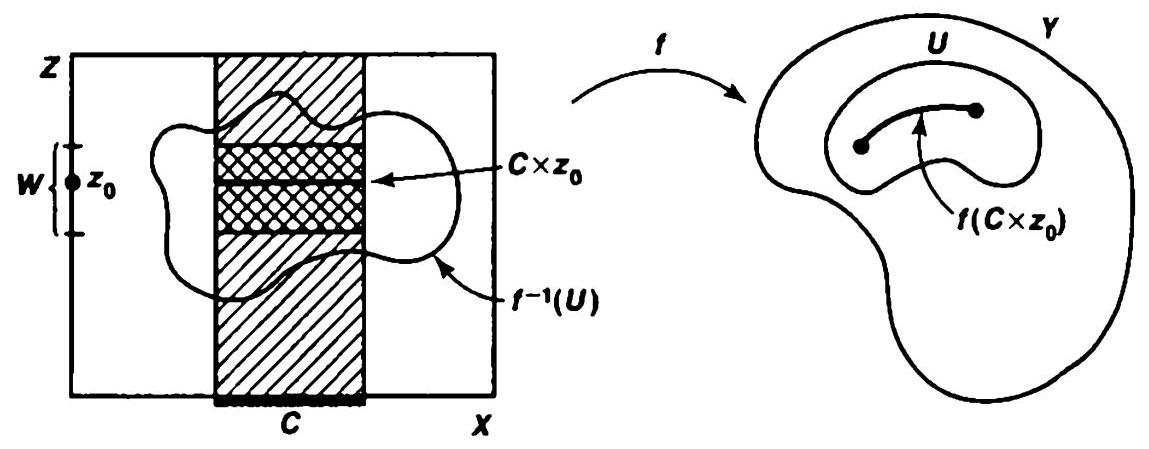
\includegraphics[width=1.0\textwidth]{images/46.2.jpg}
\end{center}
\hspace*{3em} 

Figure 46.2

We discuss briefly the connections between the compact-open topology and the concept of homotopy, which arises in algebraic topology

If \(f\) and \(g\) are continuous maps of \(X\) into \(Y\) , we say that \(f\) and \(g\) are homotopic if there is a continuous map

\[
{hX} \times  \left\lbrack  {0,1}\right\rbrack   \rightarrow  Y
\]

such that \(h\left( {x,0}\right)  = f\left( x\right)\) and \(h\left( {x,1}\right)  = g\left( x\right)\) for each \(x \in  X\) . The map \(h\) is called a homotopy between \(f\) and \(g\) .

Roughly speaking, a homotopy is a "continuous one-parameter family" of maps from \(X\) to \(Y\) More precisely, we note that a homotopy \(h\) gives rise to a map

\[
H.\left\lbrack  {0,1}\right\rbrack   \rightarrow  \mathcal{C}\left( {X,Y}\right)
\]

that assigns, to each parameter value \(t\) in \(\left\lbrack  {0,1}\right\rbrack\) , the corresponding continuous map from \(X\) to \(Y\) . Assuming that \(X\) is locally compact Hausdorff, we see that \(h\) is continuous if and only if \(H\) is continuous This means that a homotopy \(h\) between \(f\) and \(g\) corresponds precisely to a path in the function space \(\mathcal{C}\left( {X,Y}\right)\) from the point \(f\) of \(\mathcal{C}\left( {X,Y}\right)\) to the point \(g\)

We shall return to a more detailed study of homotopy in Part II of the book.
\end{proof}
\section*{Exercises}

1. Show that the sets \({B}_{C}\left( {f,\epsilon }\right)\) form a basis for a topology on \({Y}^{X}\) .

2. Prove Theorem 46.7.

3. Show that the set \(\mathcal{B}\left( {\mathbb{R},\mathbb{R}}\right)\) of bounded functions \(f : \mathbb{R} \rightarrow  \mathbb{R}\) is closed in \({\mathbb{R}}^{\mathbb{R}}\) in the uniform topology, but not in the topology of compact convergence.

4. Consider the sequence of continuous functions \({f}_{n} : \mathbb{R} \rightarrow  \mathbb{R}\) defined by

\[
{f}_{n}\left( x\right)  = x/n
\]

In which of the three topologies of Theorem 46.7 does this sequence converge? Answer the same question for the sequence given in Exercise 9 of §21.

5. Consider the sequence of functions \({f}_{n} : \left( {-1,1}\right)  \rightarrow  \mathbb{R}\) , defined by

\[
{f}_{n}\left( x\right)  = \mathop{\sum }\limits_{{k = 1}}^{n}k{x}^{k}
\]

(a) Show that \(\left( {f}_{n}\right)\) converges in the topology of compact convergence; conclude that the lumit function is continuous. (This is a standard fact about power senes.)

(b) Show that \(\left( {f}_{n}\right)\) does not converge in the uniform topology

6. Show that in the compact-open topology, \(\mathcal{C}\left( {X,Y}\right)\) is Hausdorff if \(Y\) is Hausdorff, and regular if \(Y\) is regular. [Hint: If \(\bar{U} \subset  V\) , then \(\overline{S\left( {C,U}\right) } \subset  S\left( {C,V}\right)\) .

7. Show that if \(Y\) is locally compact Hausdorff, then composition of maps

\[
\mathcal{C}\left( {X,Y}\right)  \times  \mathcal{C}\left( {Y,Z}\right)  \rightarrow  \mathcal{C}\left( {X,Z}\right)
\]

is continuous, provided the compact-open topology is used throughout. [Hint: If \(g \circ  f \in  S\left( {C,U}\right)\) , find \(V\) such that \(f\left( C\right)  \subset  V\) and \(g\left( \bar{V}\right)  \subset  U\) .\}

8. Let \({\mathcal{C}}^{\prime }\left( {X,Y}\right)\) denote the set \(\mathcal{C}\left( {X,Y}\right)\) in some topology \(\mathcal{T}\) . Show that if the evaluation map

\[
e : X \times  {\mathcal{C}}^{\prime }\left( {X,Y}\right)  \rightarrow  Y
\]

is continuous, then \(\mathcal{T}\) contains the compact-open topology. [Hint: The induced map \(E : {\mathcal{C}}^{\prime }\left( {X,Y}\right)  \rightarrow  \mathcal{C}\left( {X,Y}\right)\) is continuous. \(\}\)

9. Here is an (unexpected) application of Theorem 4611 to quotient maps. (Compare Exercise 11 of §29.)

\begin{theorem} If \(p : A \rightarrow  B\) is a quotient map and \(X\) is locally compact Hausdorff, then \({i}_{X} \times  p \cdot  X \times  A \rightarrow  X \times  B\) is a quotient map.
\end{theorem}

Proof.

(a) Let \(Y\) be the quotient space induced by \({i\chi } \times  p\) ; let \(q : X \times  A \rightarrow  Y\) be the quotient map. Show there is a bijective continuous map \(f : Y \rightarrow  X \times  B\) such that \(f \circ  q = {i}_{\chi } \times  p\) .

(b) Let \(g = {f}^{-1}\) . Let \(G : B \rightarrow  \mathcal{C}\left( {X,Y}\right)\) and \(Q : A \rightarrow  \mathcal{C}\left( {X,Y}\right)\) be the maps induced by \(g\) and \(q\) , respectively. Show that \(Q = G \circ  p\) .

(c) Show that \(Q\) is continuous; conclude that \(G\) is continuous, so that \(g\) is continuous.

*10. A space is locally compact if it can be covered by open sets each of which is contained in a compact subspace of \(X\) It is said to be \idxmath{sigma}{\(\sigma\)-compact} \(\sigma\) -compact if it can be covered by countably many such open sets.

(a) Show that if \(X\) is locally compact and second-countable, it is \(\sigma\) -compact.

(b) Let(Y, d)be a metric space. Show that if \(X\) is \(\sigma\) -compact, there is a met-nc for the topology of compact convergence on \({Y}^{X}\) such that if(Y, d)is complete, \({Y}^{X}\) is complete in this metric. [Hint: Let \({A}_{1},{A}_{2},.\) be a countable collection of compact subspaces of \(X\) whose interiors cover \(X\) . Let \({Y}_{t}\) denote the set of all functions from \({A}_{i}\) to \(Y\) , in the uniform topology. Define a homeomorphism of \({Y}^{X}\) with a closed subspace of the product space \({Y}_{1} \times  {Y}_{2} \times  \cdots \}\)

11. Let(Y, d)be a metric space; let \(X\) be a space. Define a topology on \(\mathcal{C}\left( {X,Y}\right)\) as follows: Given \(f \in  \mathcal{C}\left( {X,Y}\right)\) , and given a positive continuous function \(\delta  : X \rightarrow\)  \({\mathbb{R}}_{ + }\) on \(X\) , let

\[
B\left( {f,\delta }\right)  = \{ g \mid  d\left( {f\left( x\right) ,g\left( x\right) }\right)  < \delta \left( x\right) \text{ for all }x \in  X\} .
\]

(a) Show that the sets \(B\left( {f,\delta }\right)\) form a basis for a topology on \(\mathcal{C}\left( {X,Y}\right)\) . We call it the \idx{fine topology}.

(b) Show that the fine topology contains the uniform topology.

(c) Show that if \(X\) is compact, the fine and uniform topologies agree.

(d) Show that if \(X\) is discrete, then \(\mathcal{C}\left( {X,Y}\right)  = {Y}^{X}\) and the fine and box topologies agree.

\section*{§ 47 Ascoli’s Theorem}

Now we prove a more general version of Ascoli's theorem. It characterizes the compact subspaces of \(\mathcal{C}\left( {X,Y}\right)\) in the topology of compact convergence. The proof, however, involves all three of our standard function space topologies: the topology of pointwise convergence, the topology of compact convergence, and the uniform topology.

\begin{theorem}[Ascoli’s theorem] Let \(X\) be a space and let(Y, d)be a metric space. Give \(\mathcal{C}\left( {X,Y}\right)\) the topology of compact convergence; let \(\mathcal{F}\) be a subset of \(\mathcal{C}\left( {X,Y}\right)\) .

(a) If \(\mathcal{F}\) is equicontinuous under \(d\) and the set

\[
{\mathcal{F}}_{a} = \{ f\left( a\right)  \mid  f \in  \mathcal{F}\}
\]

has compact closure for each \(a \in  X\) , then \(\mathcal{F}\) is contained in a compact subspace of \(C\left( {X,Y}\right)\) .

(b) The converse holds if \(X\) is locally compact Hausdorff.
\end{theorem}

Proof of (a). Throughout, we give \({Y}^{X}\) the product topology, which is the same as the topology of pointwise convergence. Then \({Y}^{X}\) is a Hausdorff space. The space \(\mathcal{C}\left( {X,Y}\right)\) , which has the topology of compact convergence, is not a subspace of \({Y}^{X}\) . Let \(\mathcal{G}\) be the closure of \(\mathcal{F}\) in \({Y}^{X}\) .

Step 1. We show that \(\mathcal{G}\) is a compact subspace of \({Y}^{X}\) . Given \(a \in  X\) , let \({C}_{a}\) denote the closure of \({\mathcal{F}}_{a}\) in \(Y\) ; by hypothesis, \({C}_{a}\) is a compact subspace of \(Y\) . The set \(\mathcal{F}\) is contained in the product space

\[
\mathop{\prod }\limits_{{a \in  X}}{C}_{a}
\]

since this product by definition consists of all functions \(f : X \rightarrow  Y\) satisfying the condition \(f\left( a\right)  \in  {C}_{a}\) for all \(a\) . This product space is compact, by the Tychonoff theorem; it is a closed subspace of the product space \({Y}^{X}\) . Because \(\mathcal{G}\) equals the closure of \(\mathcal{F}\) in \({Y}^{X},\mathcal{G}\) is contained in \(\prod {C}_{a}\) , being closed, \(\mathcal{G}\) is therefore compact.

Step 2. We show that each function belonging to \(\mathcal{G}\) is continuous, and indeed that \(\mathcal{G}\) itself is equicontinuous under \(d\) .

Given \({x}_{0} \in  X\) and \(\epsilon  > 0\) , choose a neighborhood \(U\) of \({x}_{0}\) such that

(*)
\[
d\left( {f\left( x\right) ,f\left( {x}_{0}\right) }\right)  < \epsilon /3\;\text{ for all }f \in  \mathcal{F}\text{ and all }x \in  U.
\]

We shall show that \(d\left( {g\left( x\right) ,g\left( {x}_{0}\right) }\right)  < \epsilon\) for all \(g \in  \mathcal{G}\) and all \(x \in  U\) ; it follows that \(\mathcal{G}\) is equicontinuous.

Let \(g \in  \mathcal{G}\) and let \(x\) be a point of \(U\) Define \({V}_{x}\) to be the subset of \({Y}^{X}\) , open in \({Y}^{X}\) , consisting of all elements \(h\) of \({Y}^{X}\) such that

\[
\left( {* * }\right)
\]

\[
d\left( {h\left( x\right) ,g\left( x\right) }\right)  < \epsilon /3\;\text{ and }\;d\left( {h\left( {x}_{0}\right) ,g\left( {x}_{0}\right) }\right)  < \epsilon /3.
\]

Because \(g\) belongs to the closure of \(\mathcal{F}\) , the neighborhood \({V}_{x}\) of \(g\) must contain an element \(f\) of \(\mathcal{F}\) . Applying the triangle inequality to \(\left( *\right)\) and \(\left( {* * }\right)\) , it follows that \(d\left( {g\left( x\right) ,g\left( {x}_{0}\right) }\right)  < \epsilon\) , as desired.

Step 3. We show that the product topology on \({Y}^{X}\) and the compact convergence topology on \(\mathcal{C}\left( {X,Y}\right)\) coincide on the subset \(\mathcal{G}\) .

In general, the compact convergence topology is finer than the product topology. We prove that the reverse holds for the subset \(\mathcal{G}\) . Let \(g\) be an element of \(\mathcal{G}\) , and let \({B}_{C}\left( {g,\epsilon }\right)\) be a basis element for the compact convergence topology on \({Y}^{X}\) that contains \(g\) . We find a basis element \(B\) for the pointwise convergence topology on \({Y}^{X}\) that contains \(g\) such that

\[
\left\lbrack  {B \cap  \mathcal{G}}\right\rbrack   \subset  \left\lbrack  {{B}_{C}\left( {g,\epsilon }\right)  \cap  \mathcal{G}}\right\rbrack  .
\]

Using equicontinuity of \(\mathcal{G}\) and compactness of \(C\) , we can cover \(C\) by finitely many open sets \({U}_{1},\ldots ,{U}_{n}\) of \(X\) , containing points \({x}_{1},\ldots ,{x}_{n}\) , respectively, such that for each \(i\) , we have

\[
d\left( {g\left( x\right) ,g\left( {x}_{i}\right) }\right)  < \epsilon /3
\]

for \(x \in  {U}_{i}\) and \(g \in  \mathcal{G}\) . Then we define \(B\) to be the basis element for \({Y}^{X}\) defined by the equation

\[
B = \left\{  {h \mid  h \in  {Y}^{X}}\right. \text{ and }d\left( {h\left( {x}_{i}\right) ,g\left( {x}_{i}\right) }\right)  < \epsilon /3\text{ for }\left. {i = 1,\ldots ,n}\right\}  \text{ . }
\]

We show that if \(h\) is an element of \(B \cap  \mathcal{G}\) , then \(h\) belongs to \({B}_{C}\left( {g,\epsilon }\right)\) . That is, we show that \(d\left( {h\left( x\right) ,g\left( x\right) }\right)  < \epsilon\) for \(x \in  C\) . Given \(x \in  C\) , choose \(i\) so that \(x \in  {U}_{i}\) . Then

\[
d\left( {h\left( x\right) ,h\left( {x}_{i}\right) }\right)  < \epsilon /3\;\text{ and }
\]

\[
d\left( {g\left( x\right) ,g\left( {x}_{i}\right) }\right)  < \epsilon /3
\]

because \(x \in  {U}_{i}\) and \(g,h \in  \mathcal{g}\) , while

\[
d\left( {h\left( {x}_{i}\right) ,g\left( {x}_{i}\right) }\right)  < \epsilon /3
\]

because \(h \in  B\) . It follows from the triangle inequality that \(d\left( {h\left( x\right) ,g\left( x\right) }\right)  < \epsilon\) , as desired.

Step 4. We complete the proof. The set \(\mathcal{G}\) contains \(\mathcal{F}\) and is contained in \(\mathcal{C}\left( {X,Y}\right)\) . It is compact as a subspace of \({Y}^{X}\) in the product topology. By the result just proved, it is also compact as a subspace of \(\mathcal{C}\left( {X,Y}\right)\) in the compact convergence topology.

Proof of (b). Let \(\mathcal{H}\) be a compact subspace of \(\mathcal{C}\left( {X,Y}\right)\) that contains \(\mathcal{F}\) . We show that \(\mathcal{H}\) is equicontinuous and that \({\mathcal{H}}_{a}\) is compact for each \(a \in  X\) . It follows that \(\mathcal{F}\) is equicontinuous (since \(\mathcal{F} \subset  \mathcal{H}\) ), and that \({\mathcal{F}}_{a}\) lies in the compact subspace \({\mathcal{H}}_{a}\) of \(Y\) , so that \({\widetilde{\mathcal{F}}}_{a}\) is compact.

To show \({\mathcal{H}}_{a}\) is compact, consider the composite of the map

\[
j : \mathcal{C}\left( {X,Y}\right)  \rightarrow  X \times  \mathcal{C}\left( {X,Y}\right)
\]

defined by \(j\left( f\right)  = a \times  f\) , and the evaluation map

\[
e : X \times  \mathcal{C}\left( {X,Y}\right)  \rightarrow  Y
\]

given by the equation \(e\left( {x \times  f}\right)  = f\left( x\right)\) . The map \(j\) is obviously continuous, and the map \(e\) is continuous by Theorems 46.8 and 46.10. The composite \(e \circ  j\) maps \(\mathcal{H}\) to \({\mathcal{H}}_{a}\) ; since \(\mathcal{H}\) is compact, so is \({\mathcal{H}}_{a}\) .

Now we show that \(\mathcal{H}\) is equicontinuous at \(a\) , relative to the metric \(d\) . Let \(A\) be a compact subspace of \(X\) that contains a neighborhood of \(a\) . It suffices to show that the subset

\[
\mathcal{R} = \{ f \mid  A;f \in  \mathcal{H}\}
\]

of \(\mathcal{C}\left( {A,Y}\right)\) is equicontinuous at \(a\) .

Give \(\mathcal{C}\left( {A,Y}\right)\) the compact convergence topology. We show that the restriction map

\[
r : \mathcal{C}\left( {X,Y}\right)  \rightarrow  \mathcal{C}\left( {A,Y}\right)
\]

is continuous. Let \(f\) be an element of \(\mathcal{C}\left( {X,Y}\right)\) and let \(B = {B}_{C}\left( {f \mid  A,\epsilon }\right)\) be a basis element for \(\mathcal{C}\left( {A,Y}\right)\) containing \(f \mid  A\) , where \(C\) is a compact subspace of \(A\) . Then \(C\) is a compact subspace of \(X\) , and \(r\) maps the neighborhood \({B}_{C}\left( {f,\epsilon }\right)\) of \(f\) in \(\mathcal{C}\left( {X,Y}\right)\) into \(B\) .

The map \(r\) maps \(\mathcal{H}\) onto \(\mathcal{R}\) ; because \(\mathcal{H}\) is compact, so is \(\mathcal{R}\) . Now \(\mathcal{R}\) is a subspace of \(\mathcal{C}\left( {A,Y}\right)\) ; because \(A\) is compact, the compact convergence and the uniform topologies on \(\mathcal{C}\left( {A,Y}\right)\) coincide. It follows from Theorem 45.1 that \(\mathcal{R}\) is totally bounded in the uniform metric on \(\mathcal{C}\left( {A,Y}\right)\) ; then Lemma 45.2 implies that \(\mathcal{R}\) is equicontinuous relative to \(d\) .

An even more general version of Ascoli's theorem may be found in 		\cite{Kelley1991} or 		\cite{Willard1970}. There it is not assumed that \(Y\) is a metric space, but only that it has what is called a uniform structure, which is a generalization of the notion of metric.

Ascoli's theorem has many applications in analysis, but these lie outside the scope of this book. See 		\cite{KolmogorovFomin1957} for several such applications.

\section*{Exercises}

1. Which of the following subsets of \(\mathcal{C}\left( {\mathbb{R},\mathbb{R}}\right)\) are pointwise bounded? Which are equicontinuous?

(a) The collection \(\left\{  {f}_{n}\right\}\) , where \({f}_{n}\left( x\right)  = x + \sin {nx}\) .

(b) The collection \(\left\{  {g}_{n}\right\}\) , where \({g}_{n}\left( x\right)  = n + \sin x\) .

(c) The collection \(\left\{  {h}_{n}\right\}\) , where \({h}_{n}\left( x\right)  = {\left| x\right| }^{1/n}\) .

(d) The collection \(\left\{  {k}_{n}\right\}\) , where \({k}_{n}\left( x\right)  = n\sin \left( {x/n}\right)\) .

2. Prove the following

\begin{theorem} If \(X\) is a locally compact Hausdorff space, then a subspace \(\mathcal{F}\) of \(\mathcal{C}\left( {X,{\mathbb{R}}^{n}}\right)\) in the topology of compact convergence has compact closure if and only if \(\mathcal{F}\) is pointwise bounded and equicontinuous under either of the standard metrics on \({\mathbb{R}}^{n}\) .
\end{theorem}

3. Show that the general version of Ascoli’s theorem implies the classical version (Theorem 45.4) when \(X\) is Hausdorff.

4. Prove the following:

\begin{theorem}[Arzela’s theorem, general version] Let \(X\) be a Hausdorff space that is \(\sigma\) -compact; let \({f}_{n}\) be a sequence of functions \({f}_{n} : X \rightarrow  {\mathbb{R}}^{k}\) . If the collection \(\left\{  {f}_{n}\right\}\) is pointwise bounded and equicontinuous, then the sequence \({f}_{n}\) has a subsequence that converges, in the topology of compact convergence, to a continuous function.
\end{theorem}

\{Hint: Show \(\mathcal{C}\left( {X,{\mathbb{R}}^{k}}\right)\) is first-countable.\}

5. Let(Y, d)be a metric space; let \({f}_{n} : X \rightarrow  Y\) be a sequence of continuous functions; let \(f : X \rightarrow  Y\) be a function (not necessarily continuous). Suppose \({f}_{n}\) converges to \(f\) in the topology of pointwise convergence. Show that if \(\left\{  {f}_{n}\right\}\) is equicontinuous, then \(f\) is continuous and \({f}_{n}\) converges to \(f\) in the topology of compact convergence.